\documentclass{article}

% Packages for setting up page margins
\usepackage[margin=1in]{geometry}

\usepackage{graphicx, setspace, amsmath, mathtools, amssymb, url, float}
\setlength{\parskip}{2mm}
\graphicspath{ {./images/} }

% Title
\title{CS451 Introduction to Parallel and Distributed Computing - Assignment 4}
\author{Batkhishig Dulamsurankhor - A20543498}
\date{\today} % Use \date{} for no date

\begin{document}

\maketitle

\begin{enumerate}
  \item Screen shot of the apps working for part b. Screenshot of the hello world working in part a.
  \begin{enumerate}
    \item part a.
    \begin{figure}[H]
      \centering
      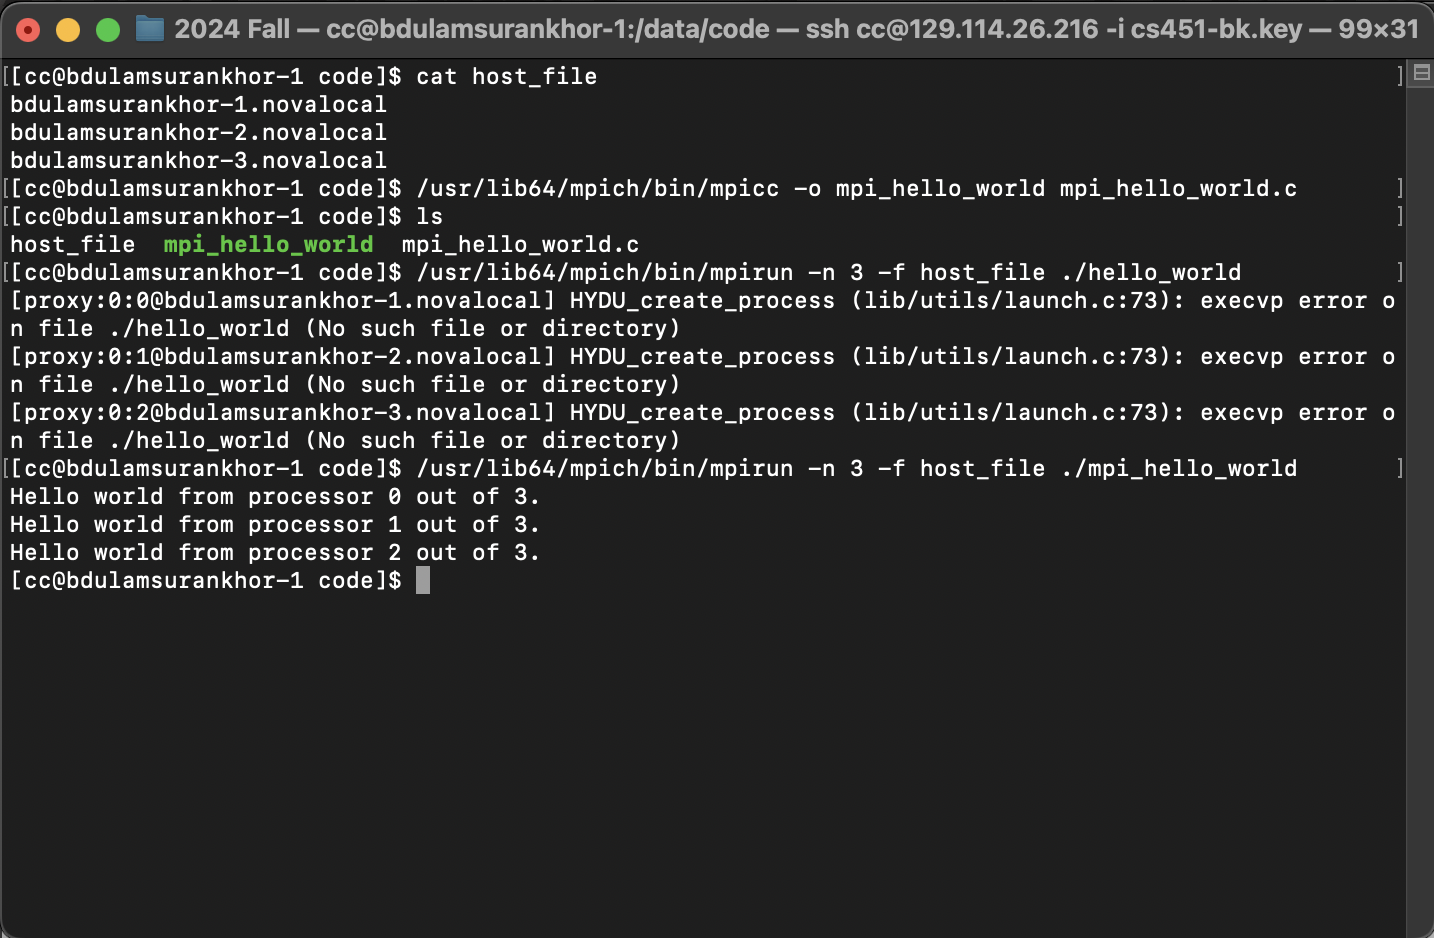
\includegraphics[width=\textwidth]{image2.png}
      \caption{Screenshot of the hello world working in part a.}
    \end{figure}
    
    \item part b.
    \begin{enumerate}
      \item Adjust hello world so that after you type in your name once, when prompted by the manager node, every node salutes you, using the name you typed in.
      \begin{figure}[H]
        \centering
        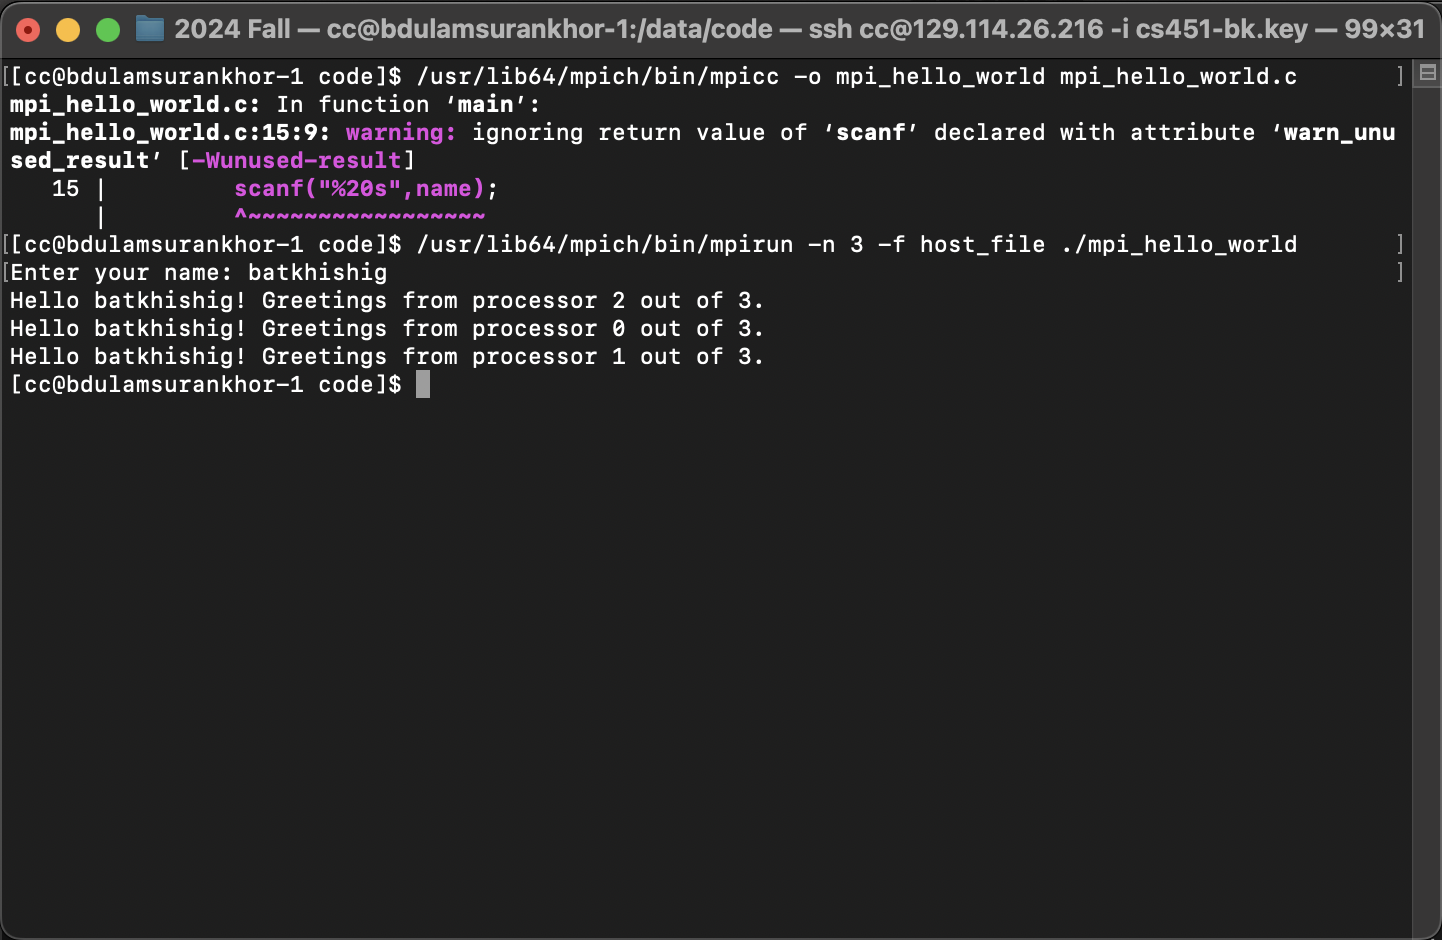
\includegraphics[width=\textwidth]{image3.png}
        \caption{Screenshot of part b, q1.}
      \end{figure}
      \item We measure the wall clock time using time mpirun in the broadcasting of an array of doubles.
      To avoid typing in the dimension n, either define n as a constant in the program or redirect the input from a file that contains n.
      For increasing number of processes and n, investigate how the wall clock time grows. Run N as 2,4,8,16,32.
      \begin{figure}[H]
        \centering
        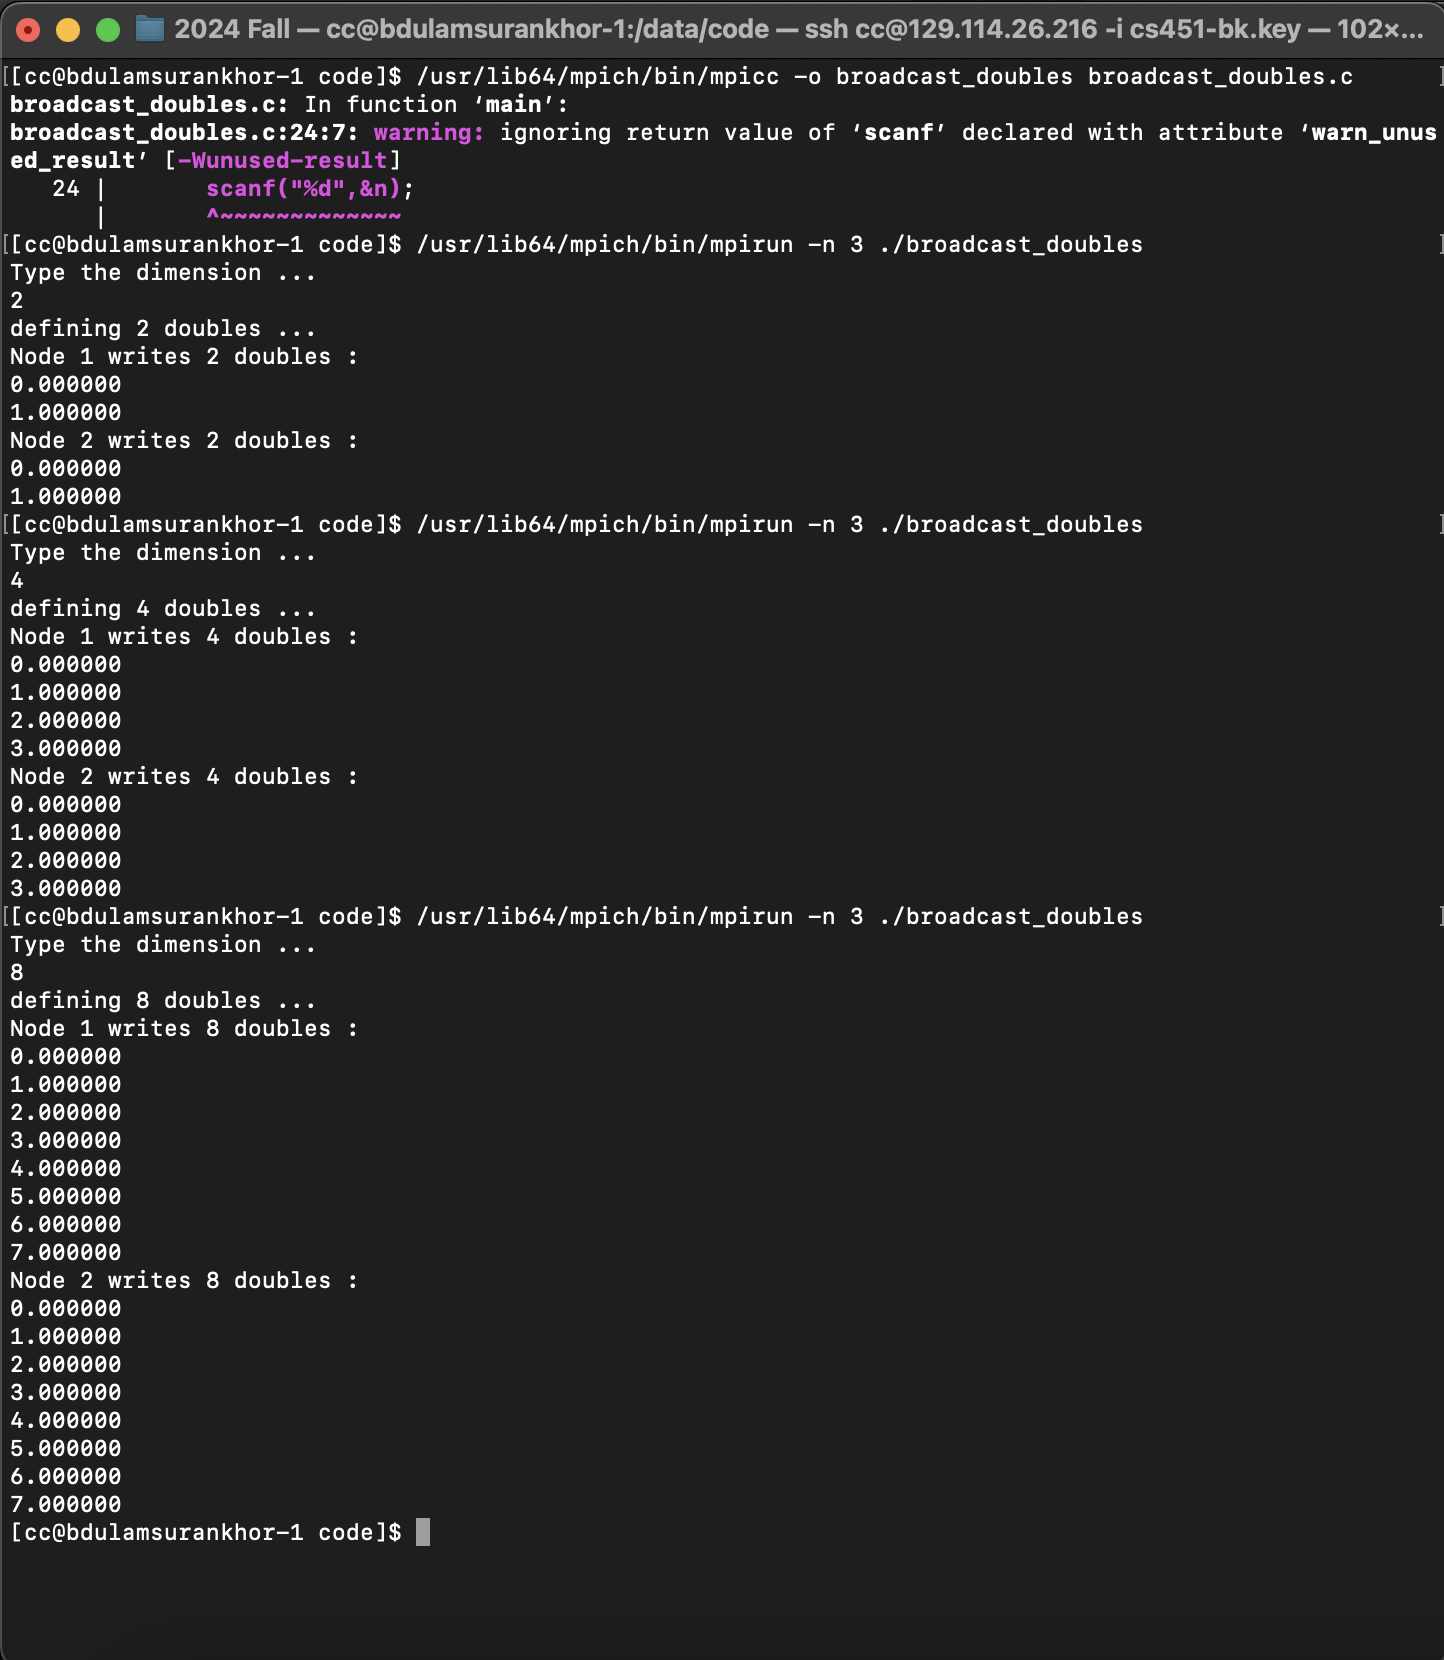
\includegraphics[width=\textwidth]{image4.png}
        \caption{Screenshot of part b, q2. n=2,4,8}
      \end{figure}
      \begin{figure}[H]
        \centering
        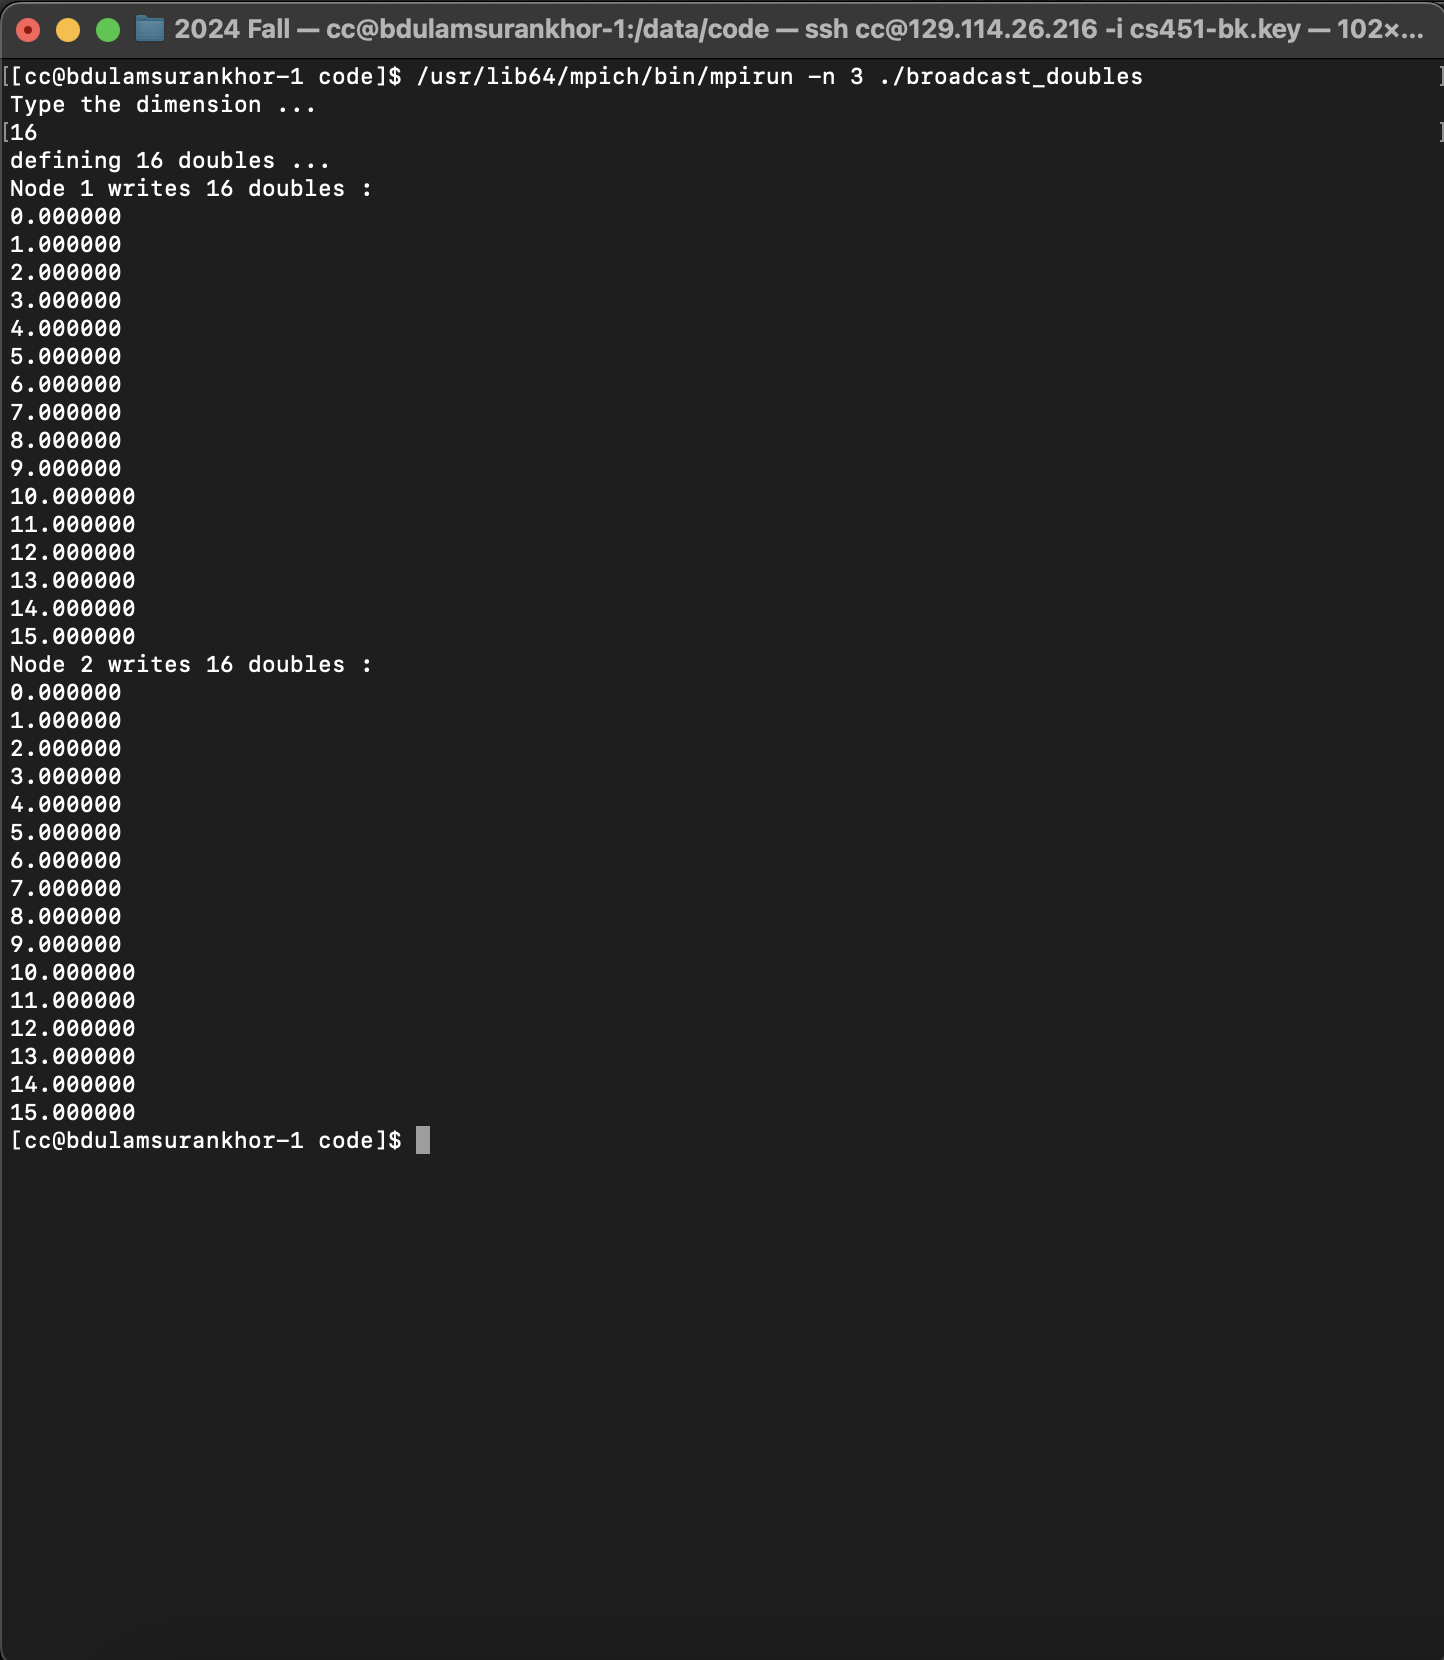
\includegraphics[width=\textwidth]{image5.png}
        \caption{Screenshot of part b, q2. n=16}
      \end{figure}
      \begin{figure}[H]
        \centering
        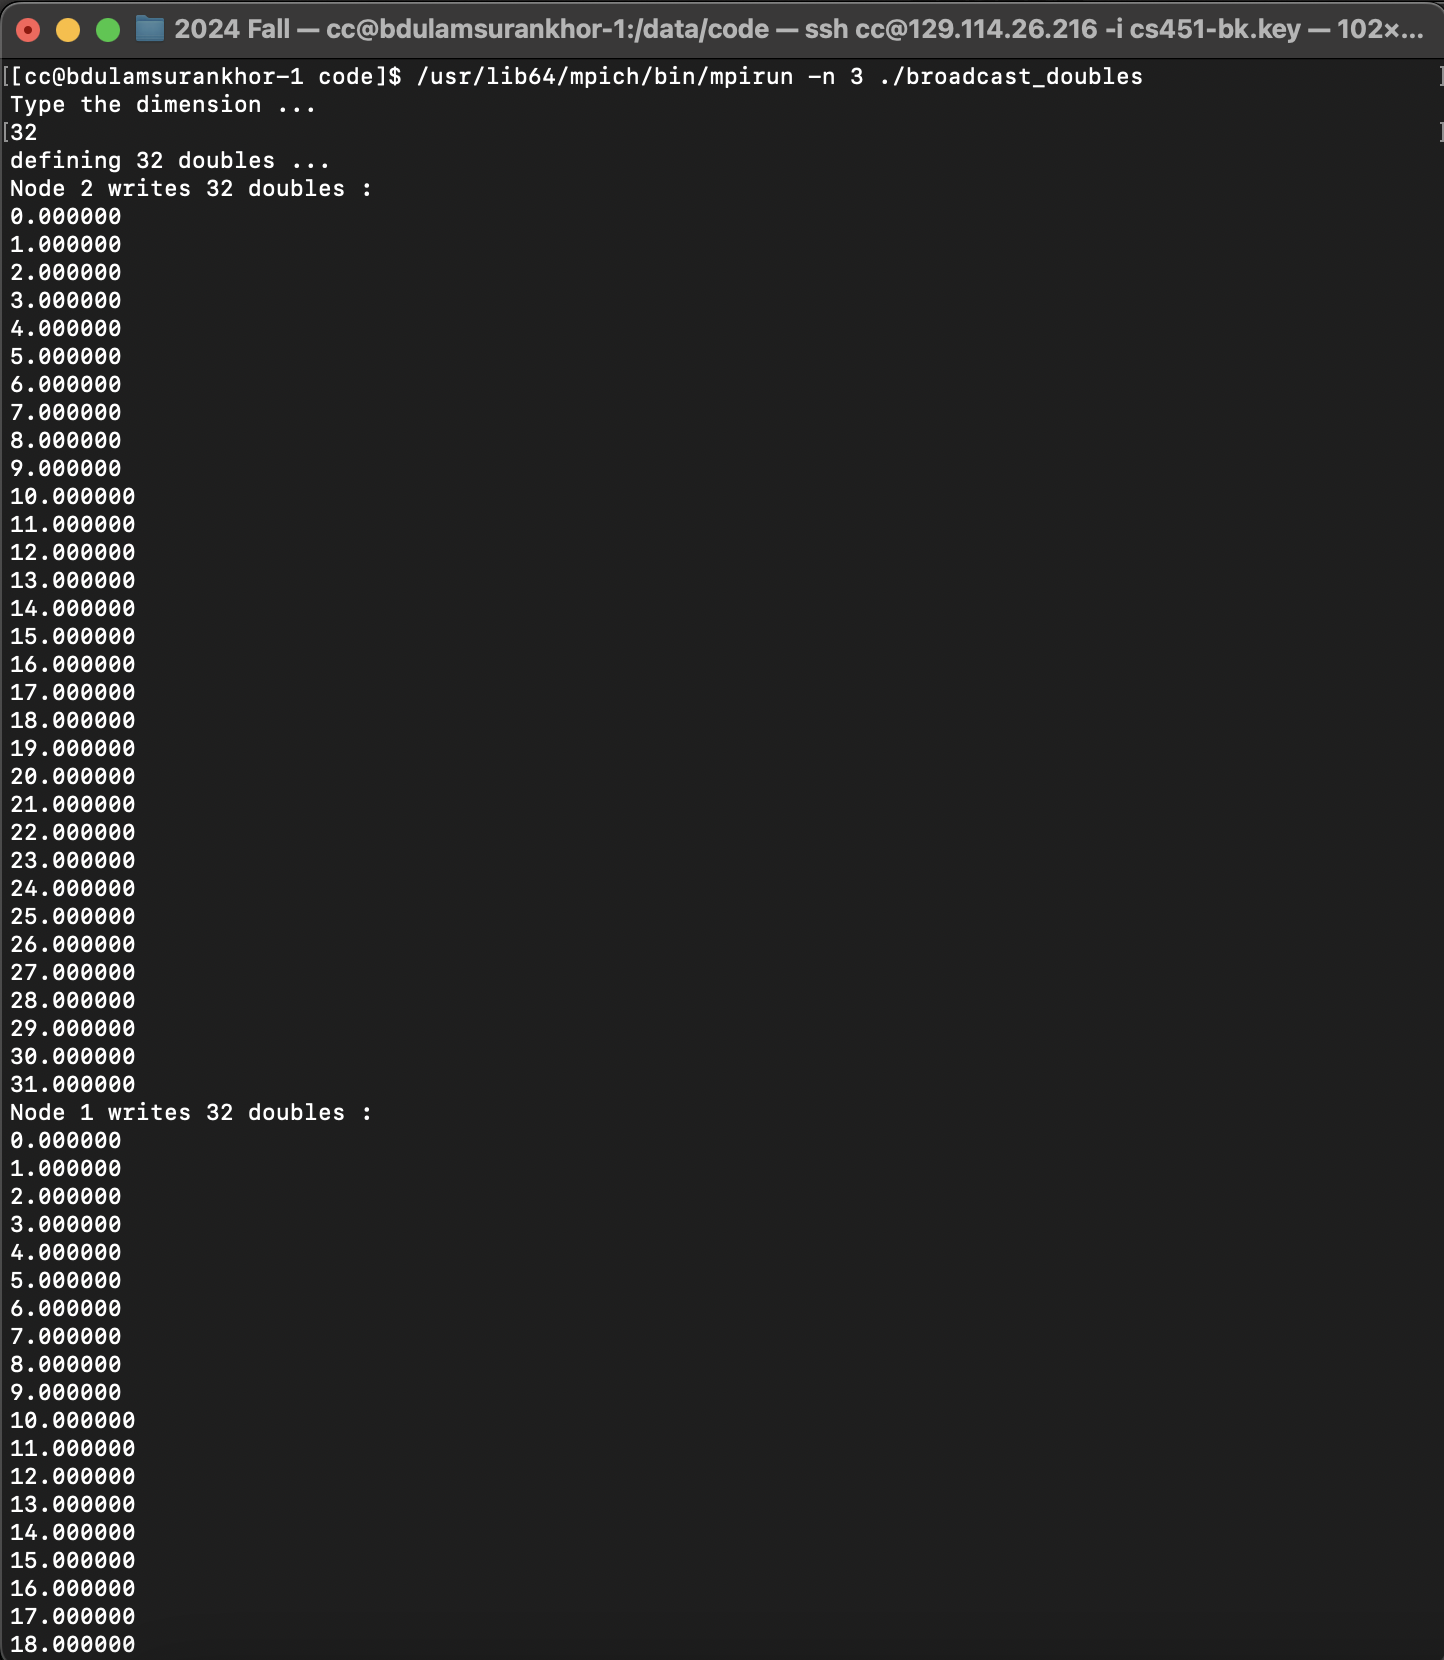
\includegraphics[width=\textwidth]{image6.png}
        \caption{Screenshot of part b, q2. n=32}
      \end{figure}
      \begin{figure}[H]
        \centering
        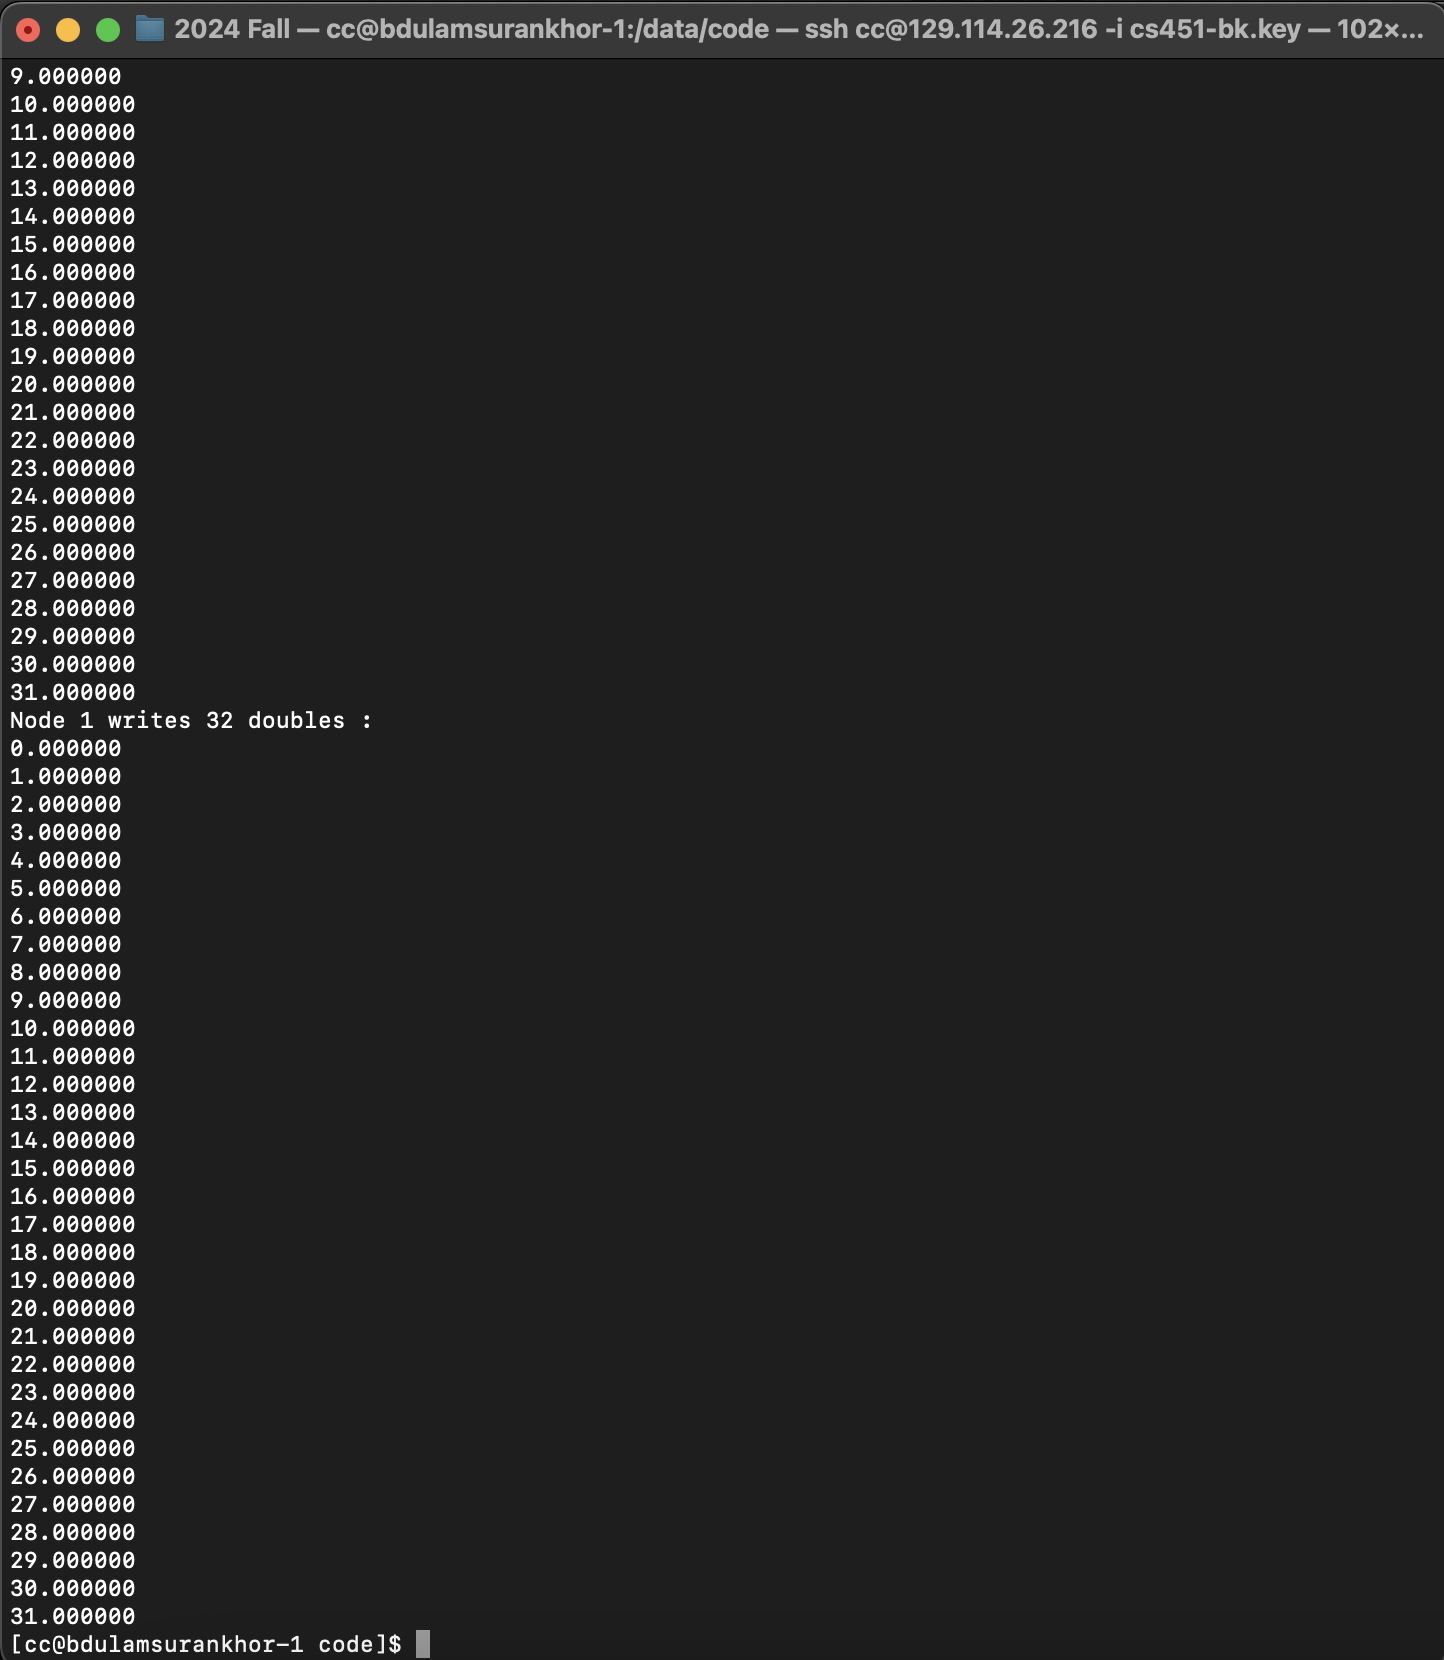
\includegraphics[width=\textwidth]{image7.png}
        \caption{Screenshot of part b, q2. n=32}
      \end{figure}
      \item Compile and run both static\_loaddist.c and dynamic\_loaddist.c and compare the runtimes. Run N as 2,4,8,16,32.
      \begin{figure}[H]
        \centering
        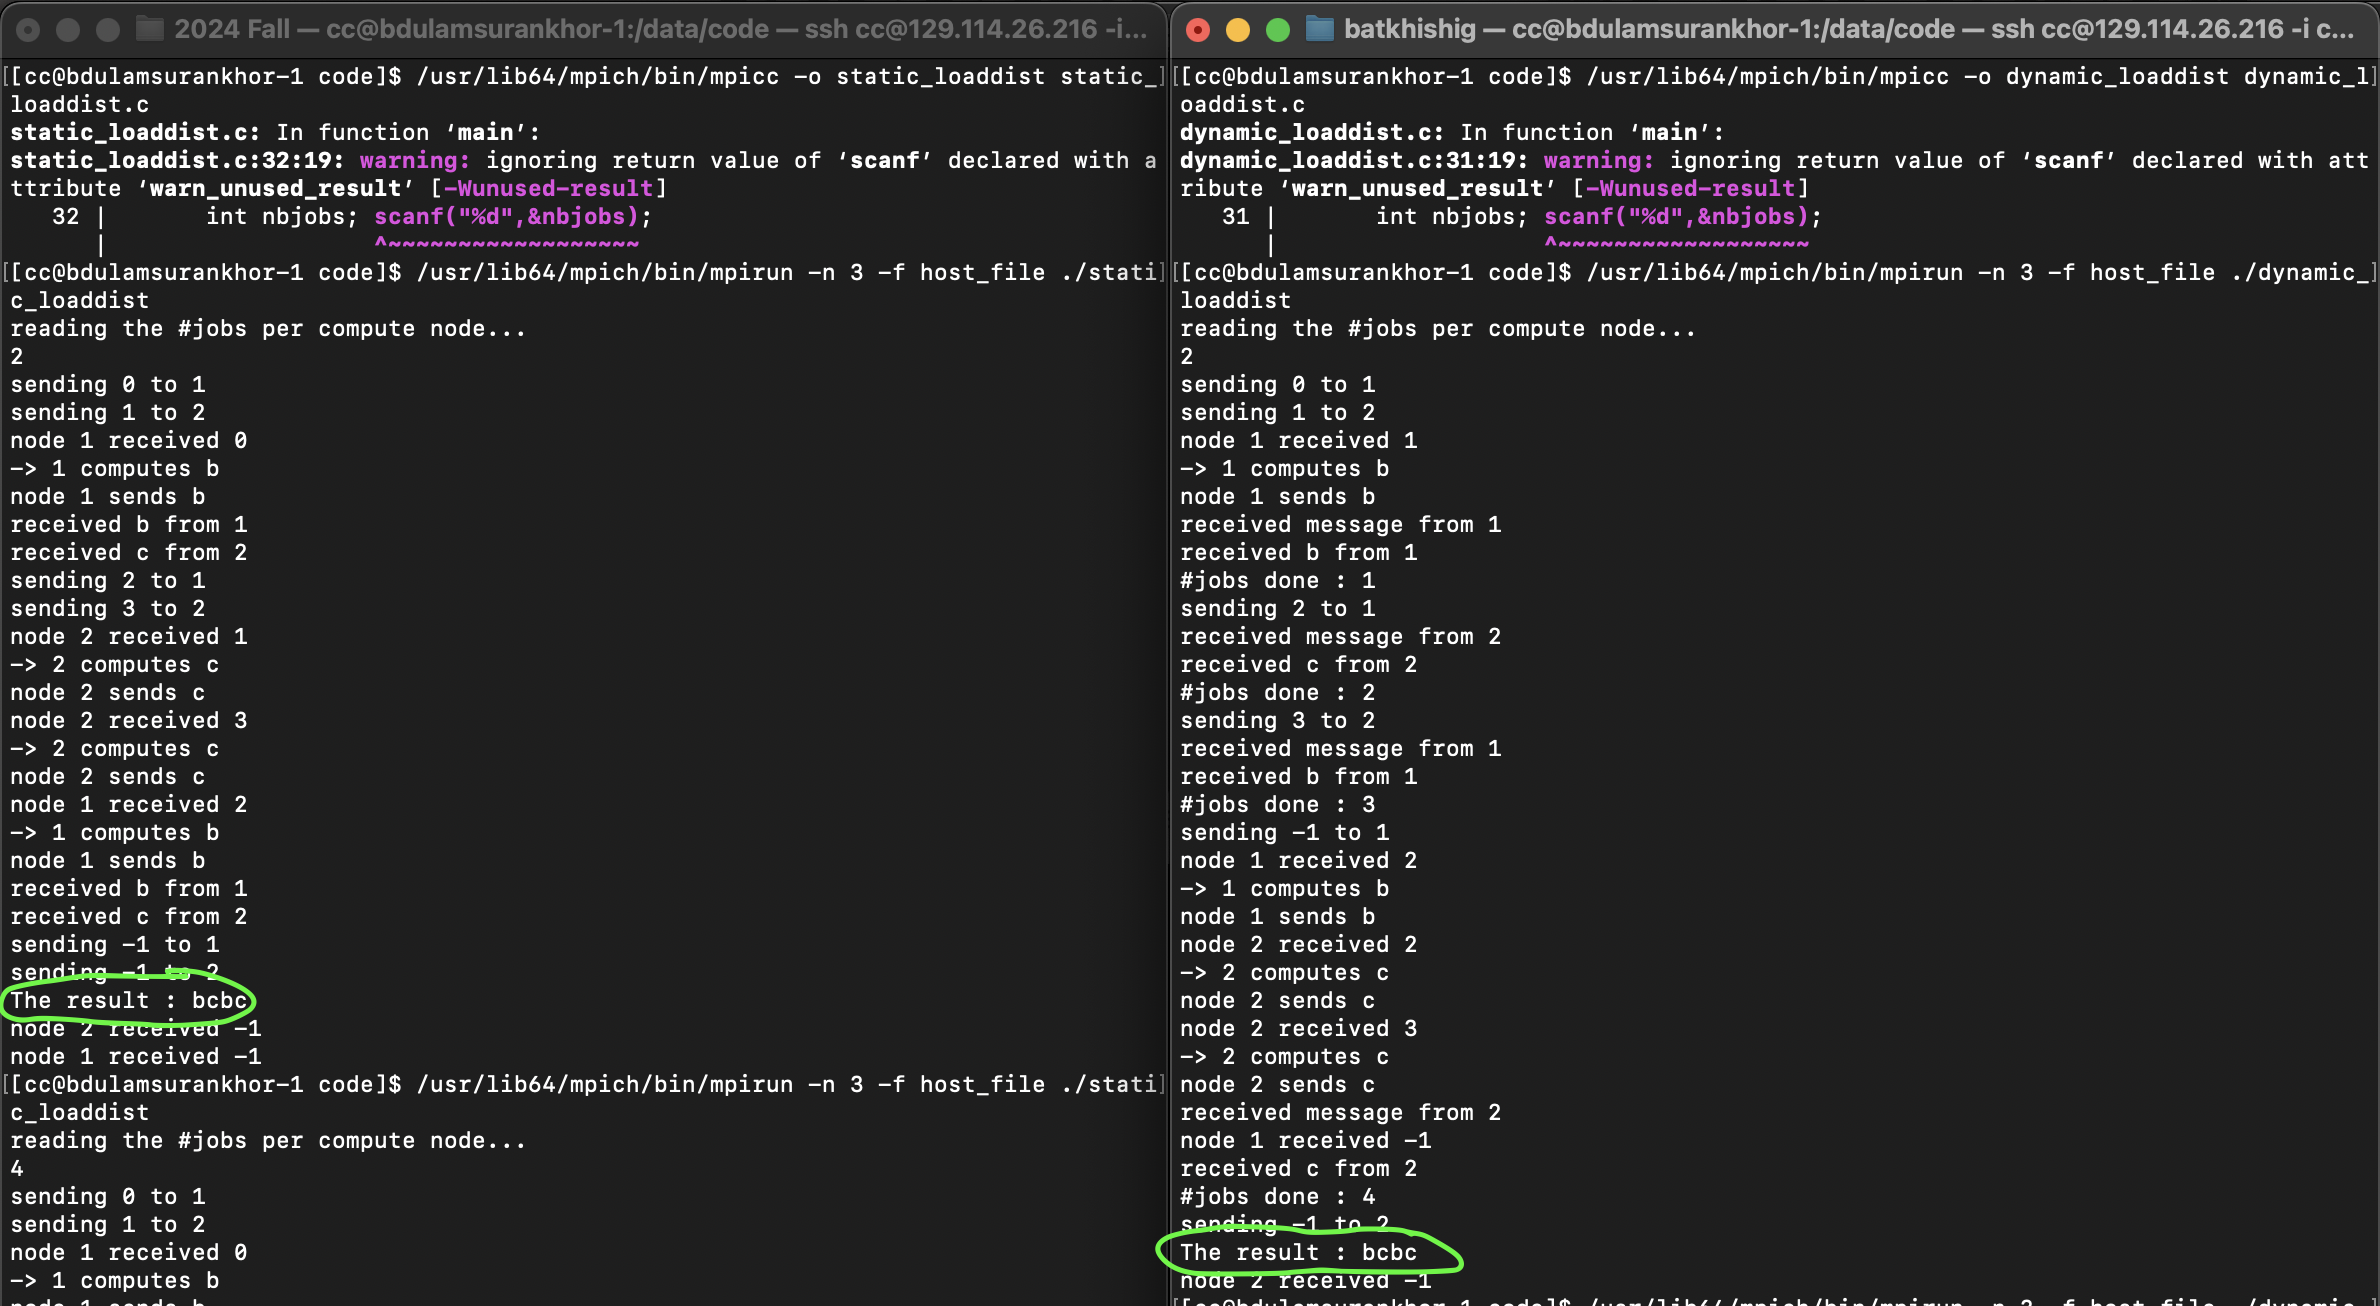
\includegraphics[width=\textwidth]{image8.png}
        \caption{Screenshot of part b, q3. n=2}
      \end{figure}
      \begin{figure}[H]
        \centering
        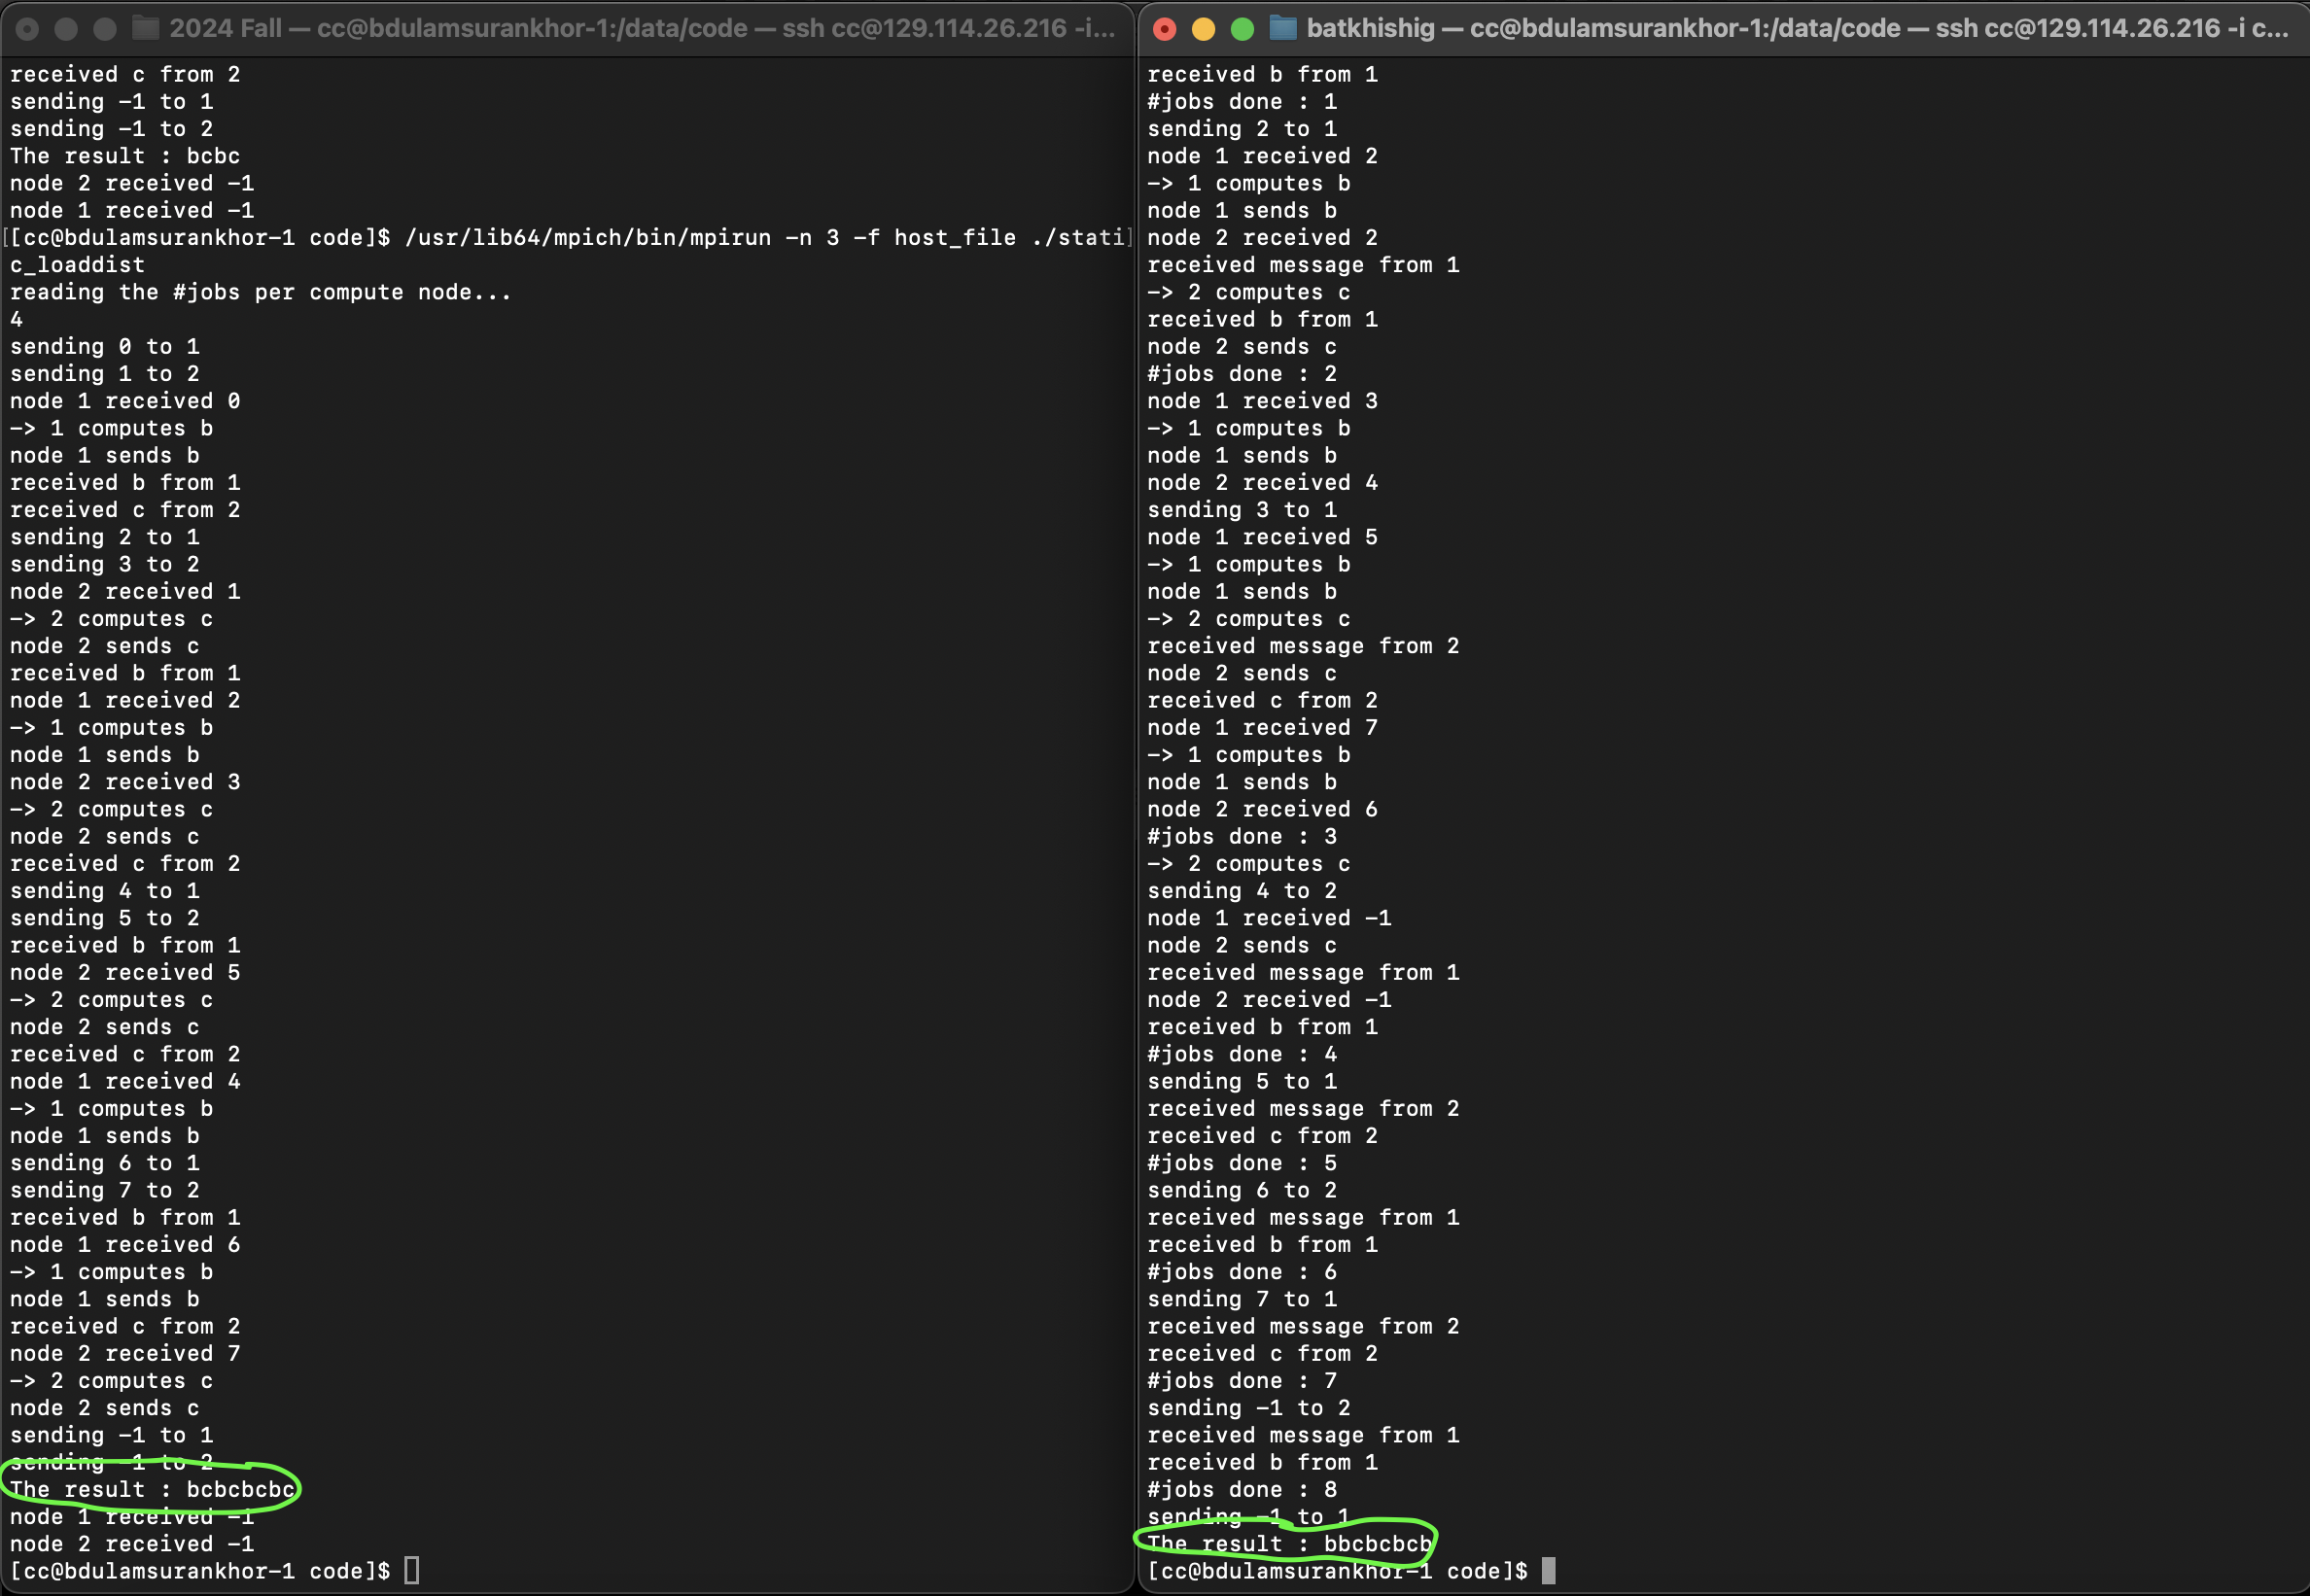
\includegraphics[width=\textwidth]{image9.png}
        \caption{Screenshot of part b, q3. n=4}
      \end{figure}
      \begin{figure}[H]
        \centering
        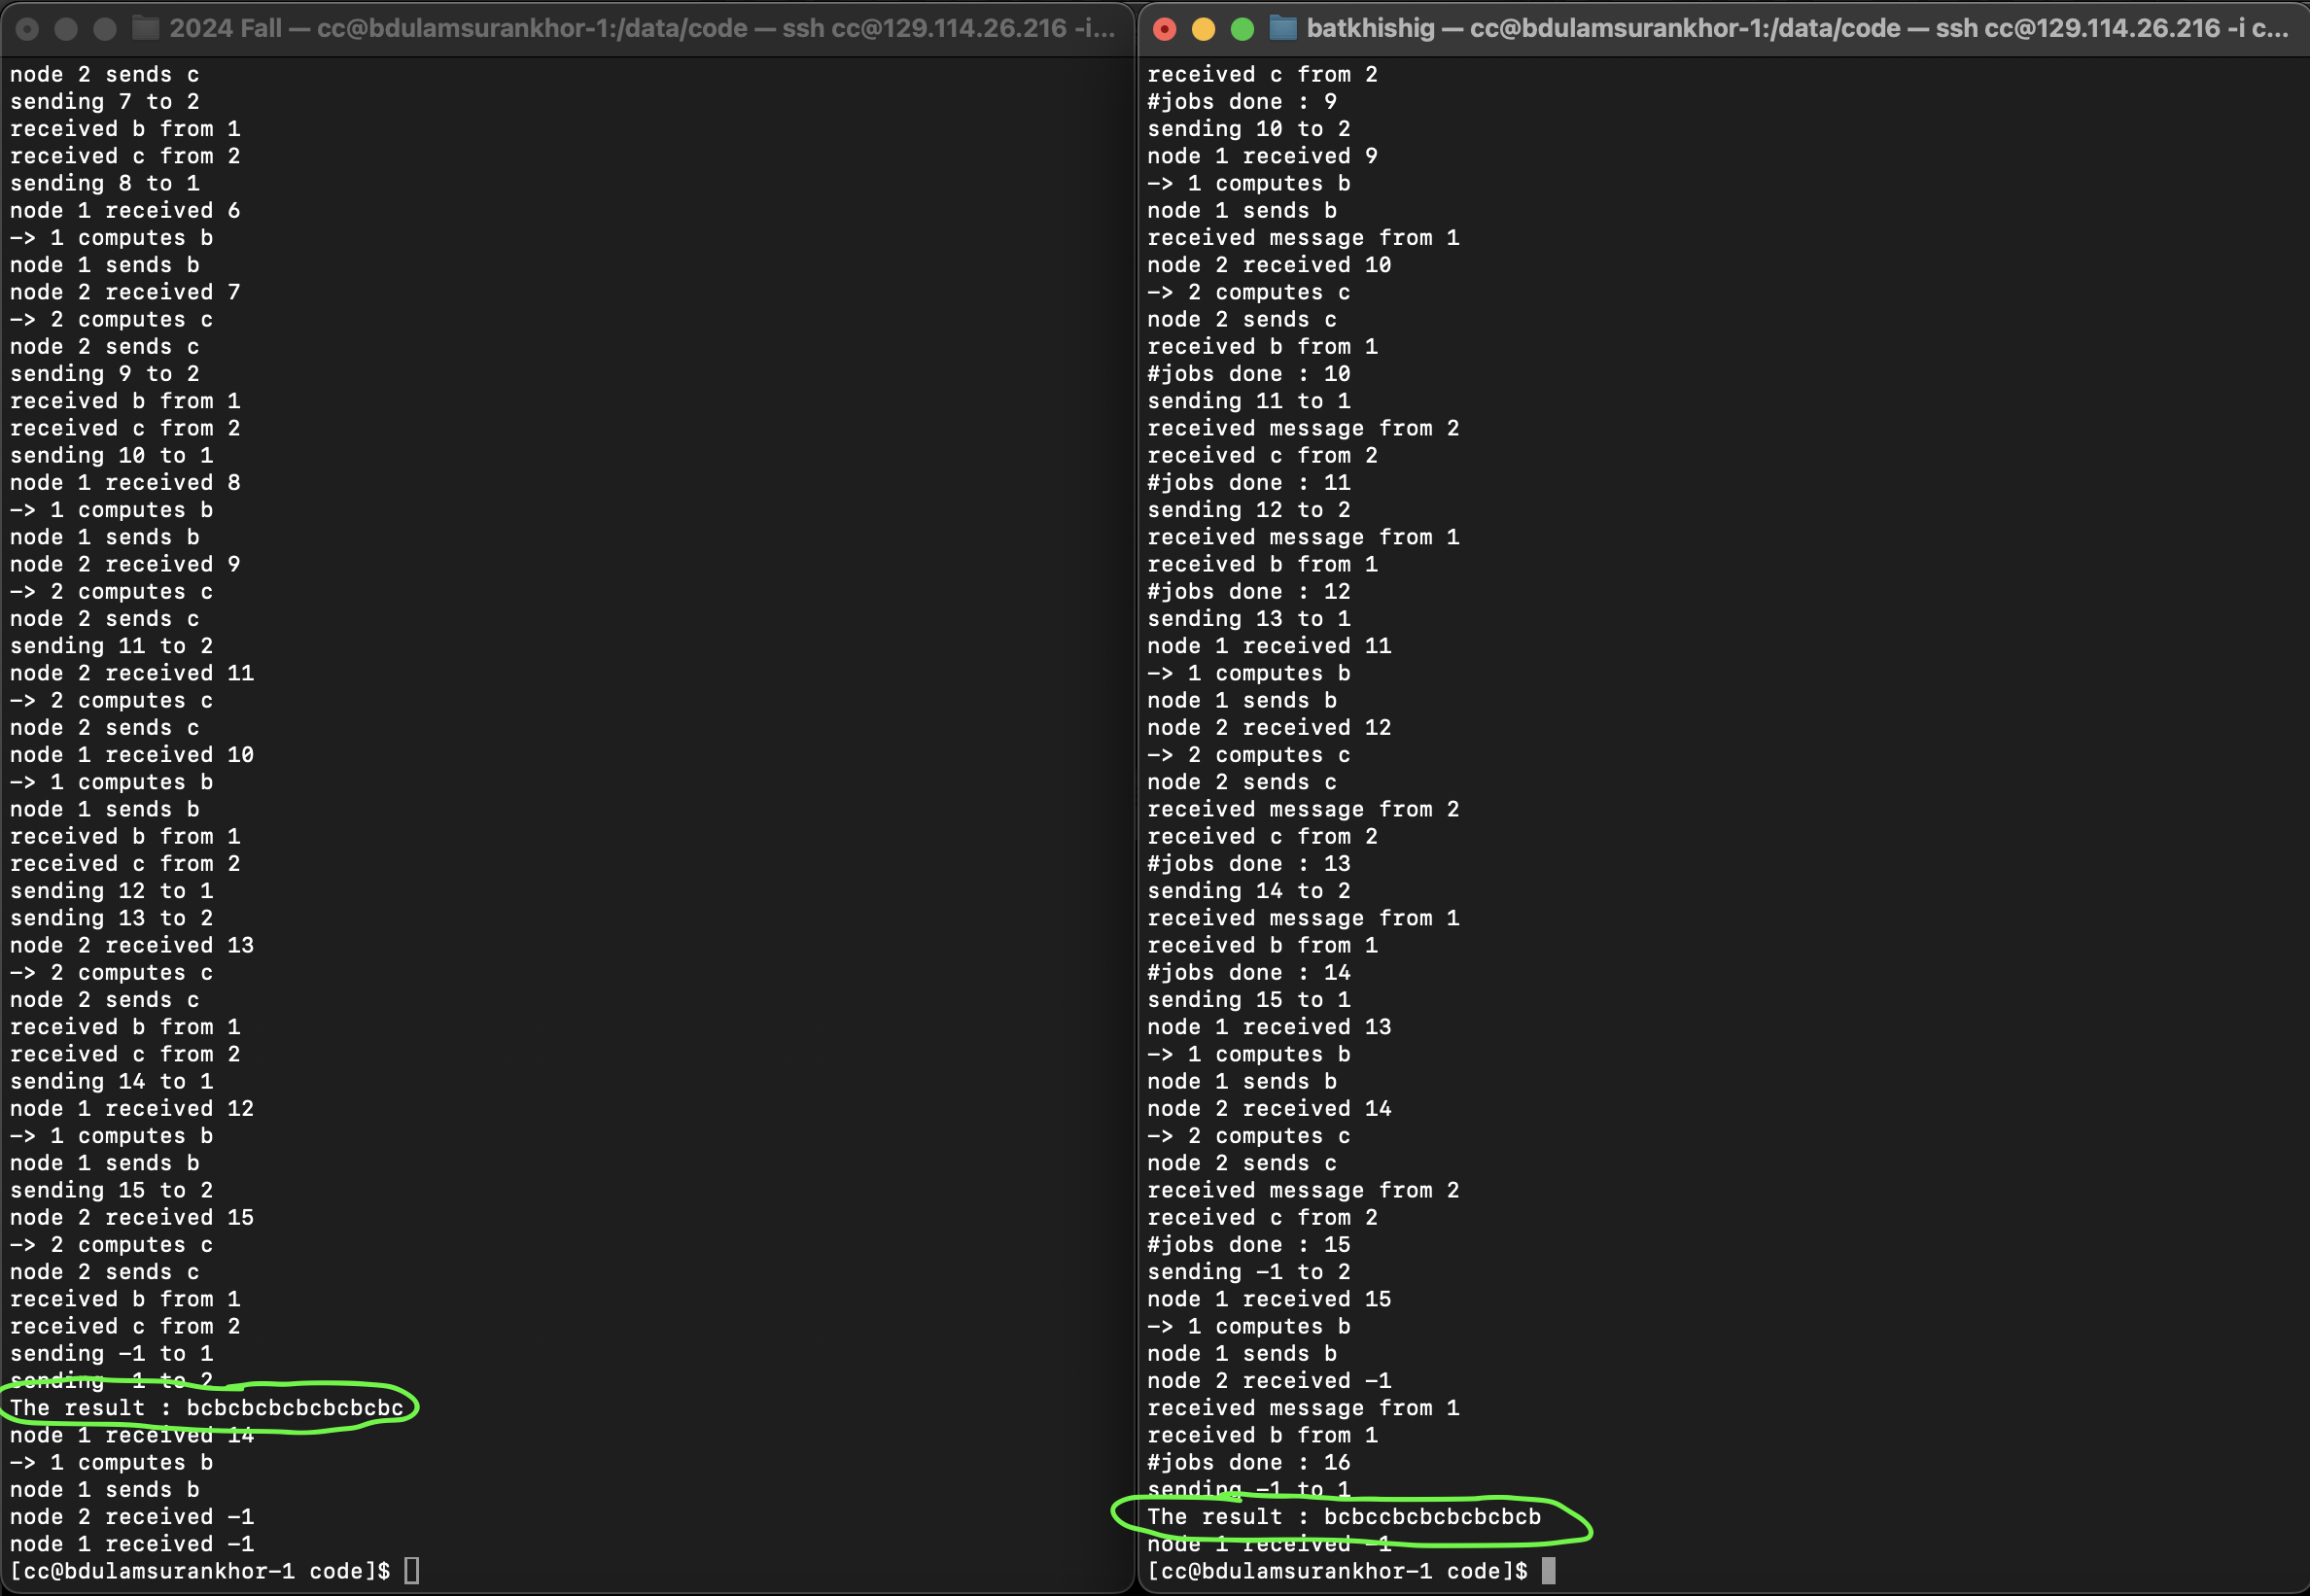
\includegraphics[width=\textwidth]{image10.png}
        \caption{Screenshot of part b, q3. n=8}
      \end{figure}
      \begin{figure}[H]
        \centering
        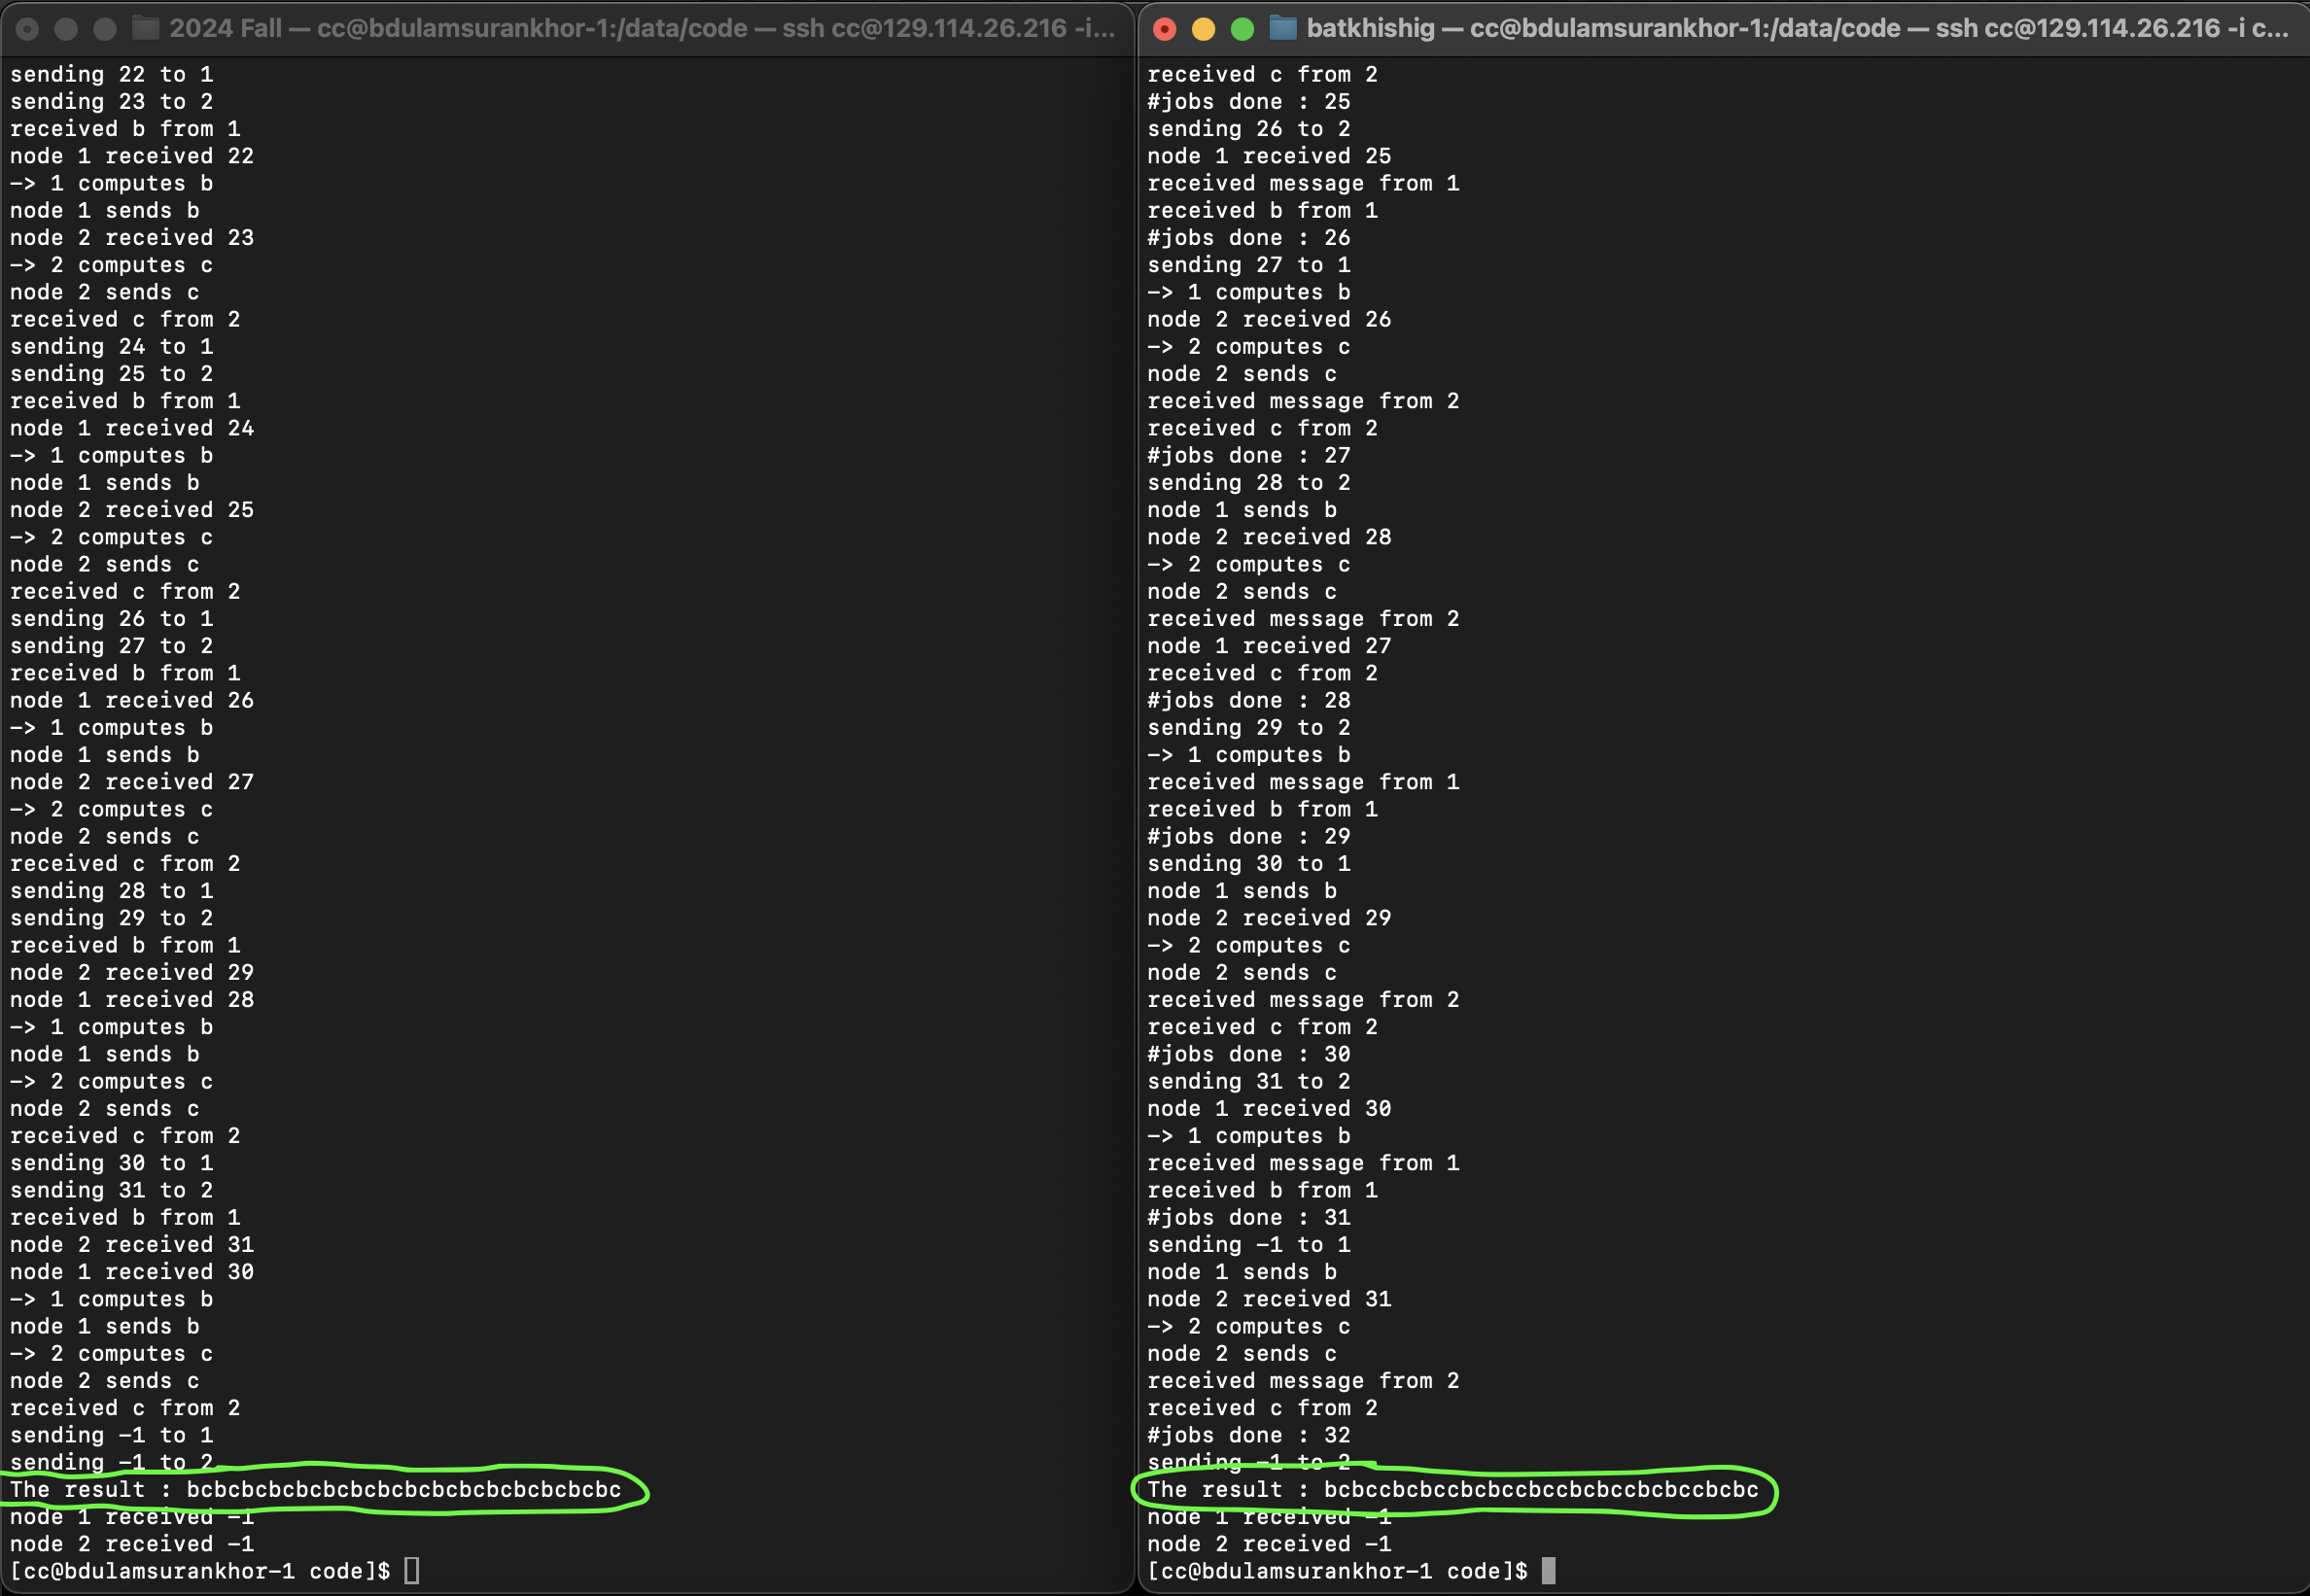
\includegraphics[width=\textwidth]{image11.png}
        \caption{Screenshot of part b, q3. n=16}
      \end{figure}
      \begin{figure}[H]
        \centering
        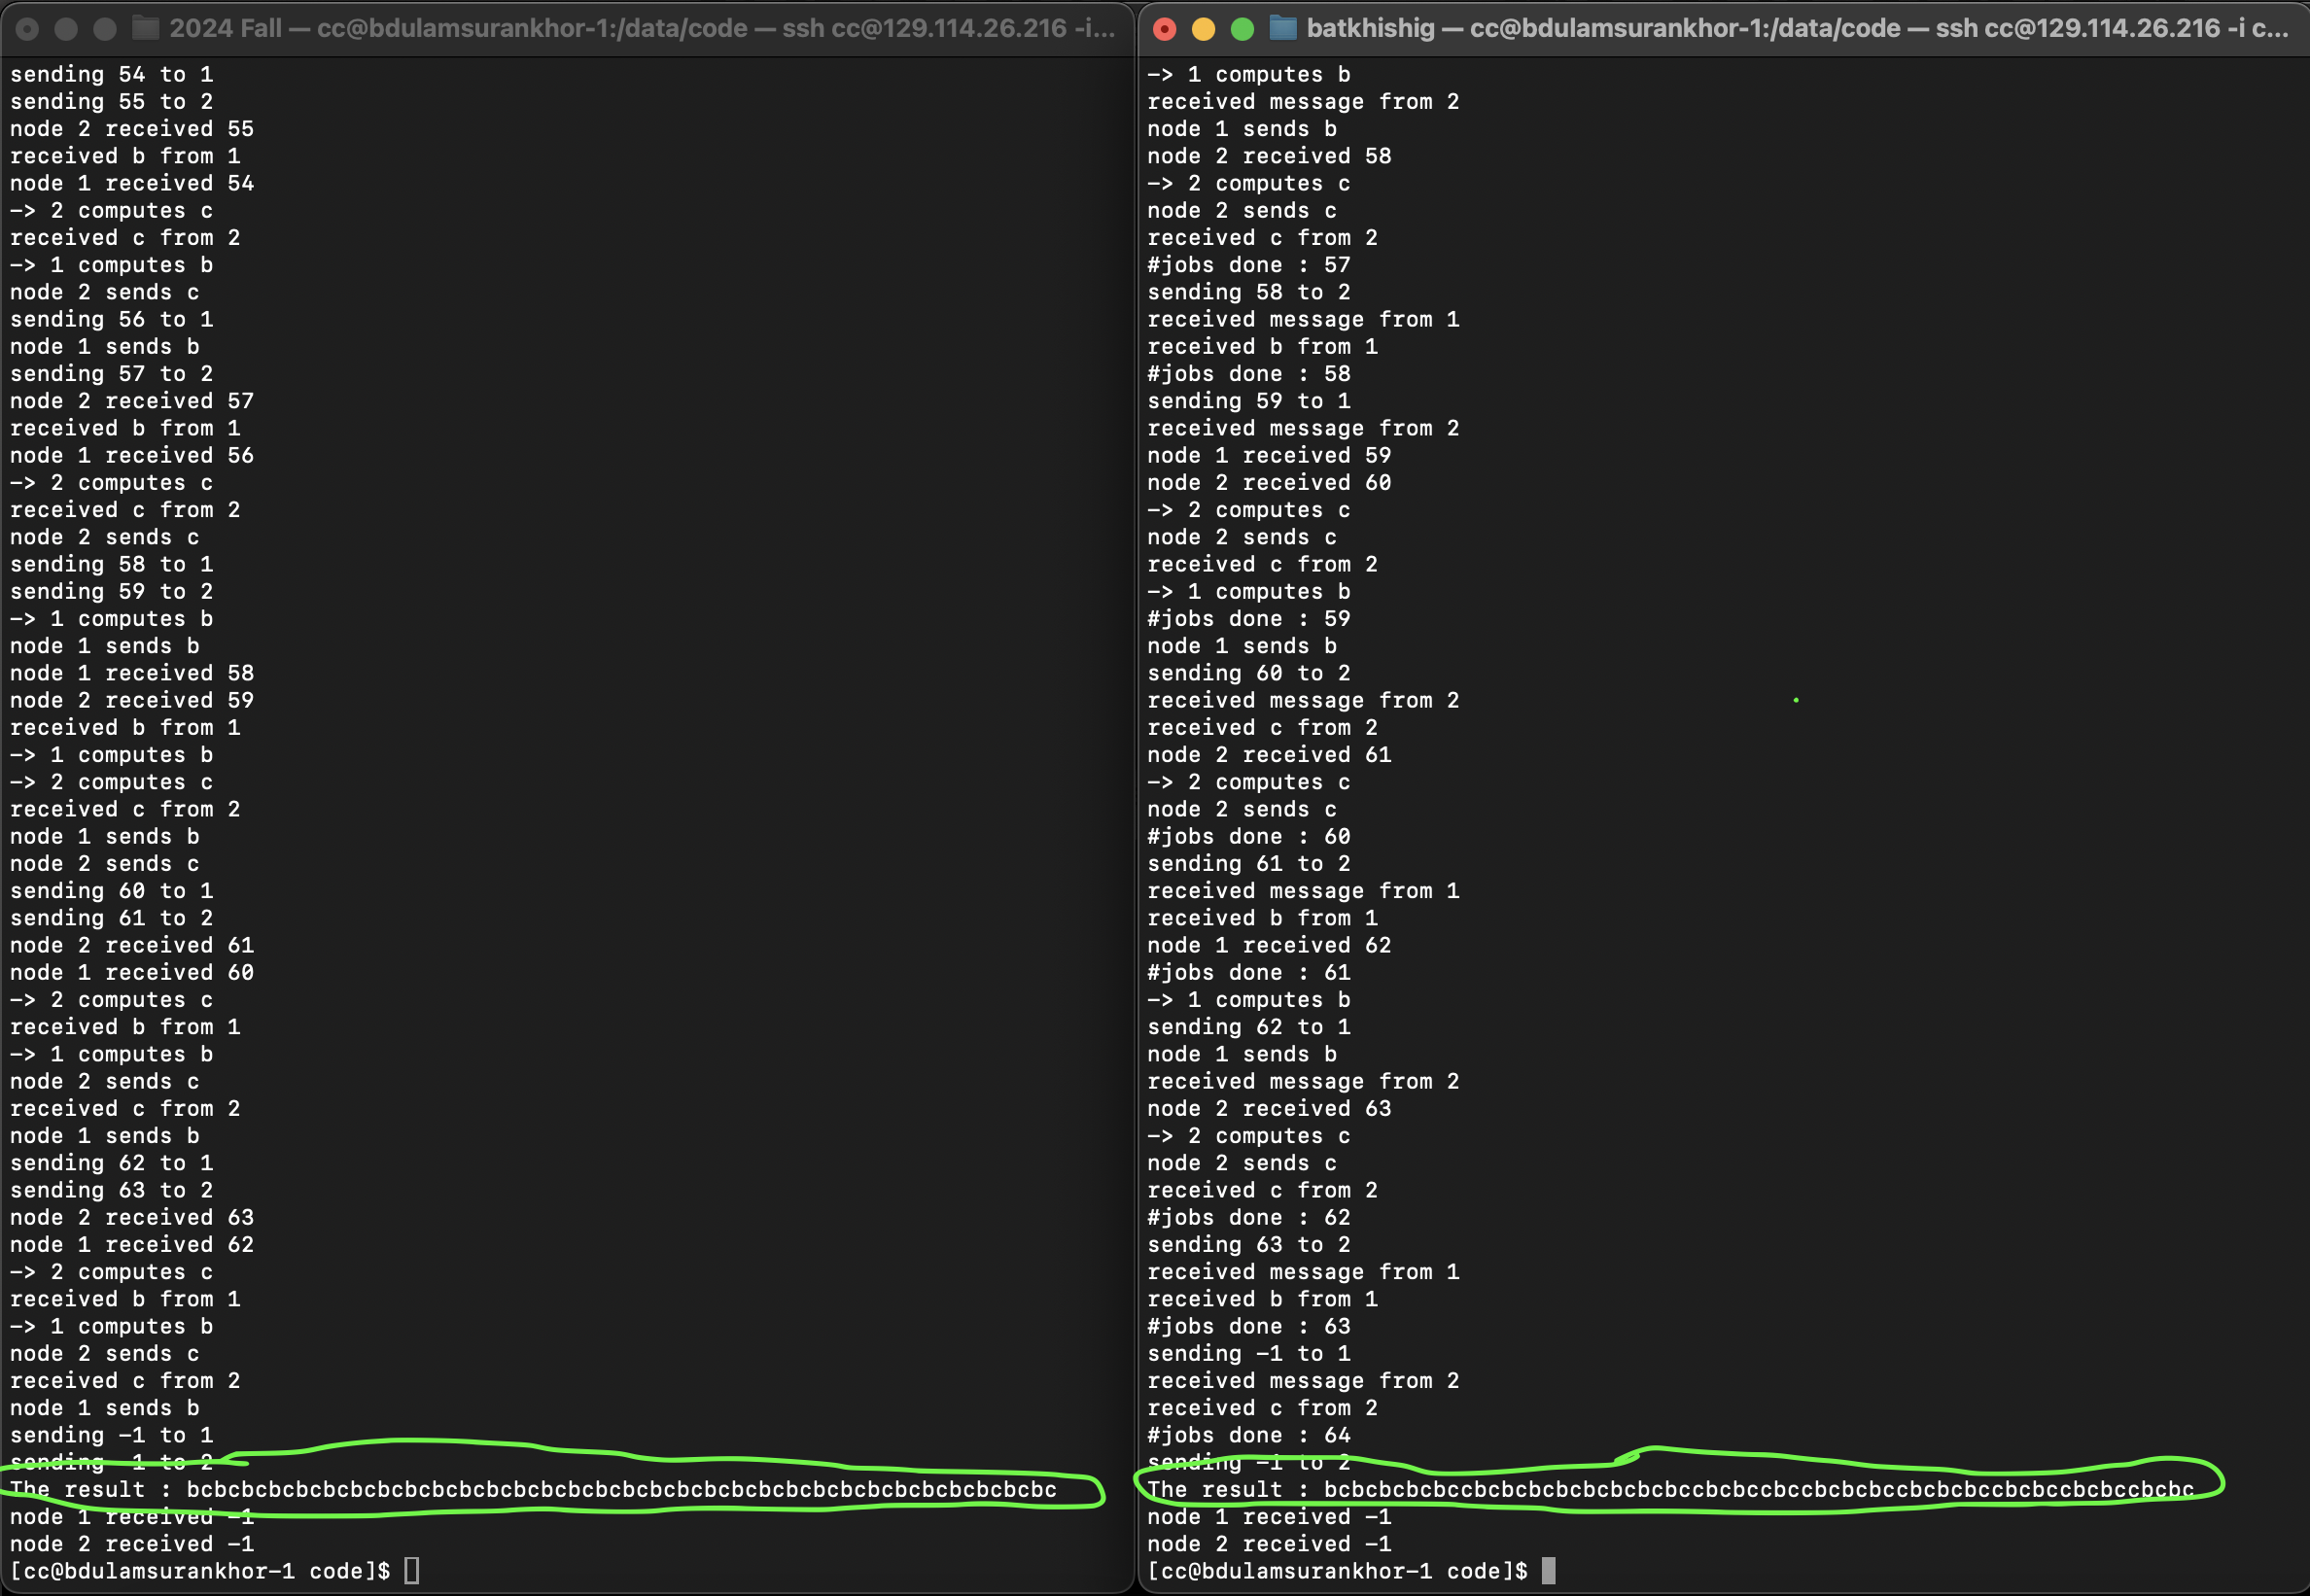
\includegraphics[width=\textwidth]{image12.png}
        \caption{Screenshot of part b, q3. n=32}
      \end{figure}
      \item Adjust parallel\_sum.c to go to 200 instead of 100 and adjust it to work for p processors where the dimension n of the array is a multiple of p.
      In other words, so if you have N = 3 or 6 , it'll work correctly.
      \begin{figure}[H]
        \centering
        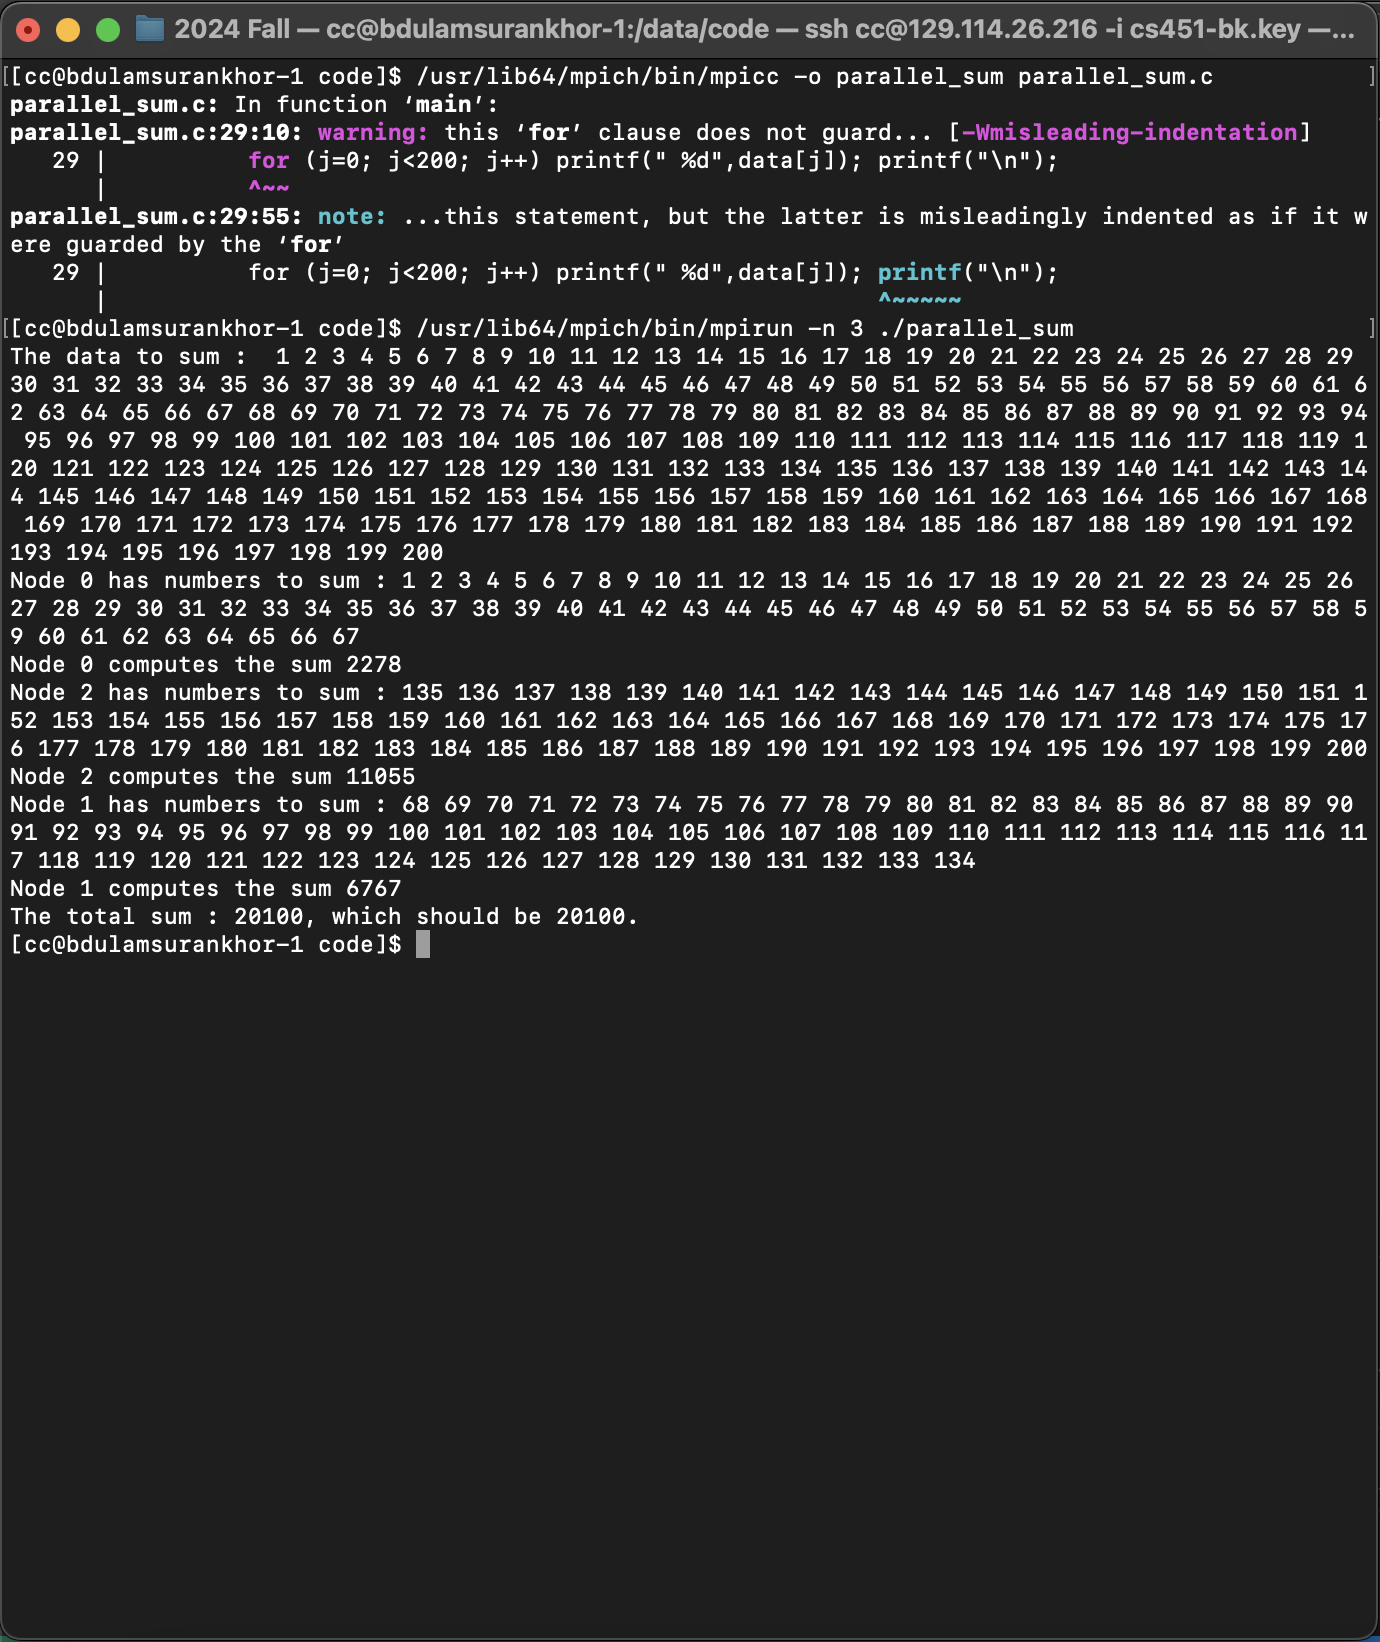
\includegraphics[width=\textwidth]{image13.png}
        \caption{Screenshot of part b, q4. n=3}
      \end{figure}
      \begin{figure}[H]
        \centering
        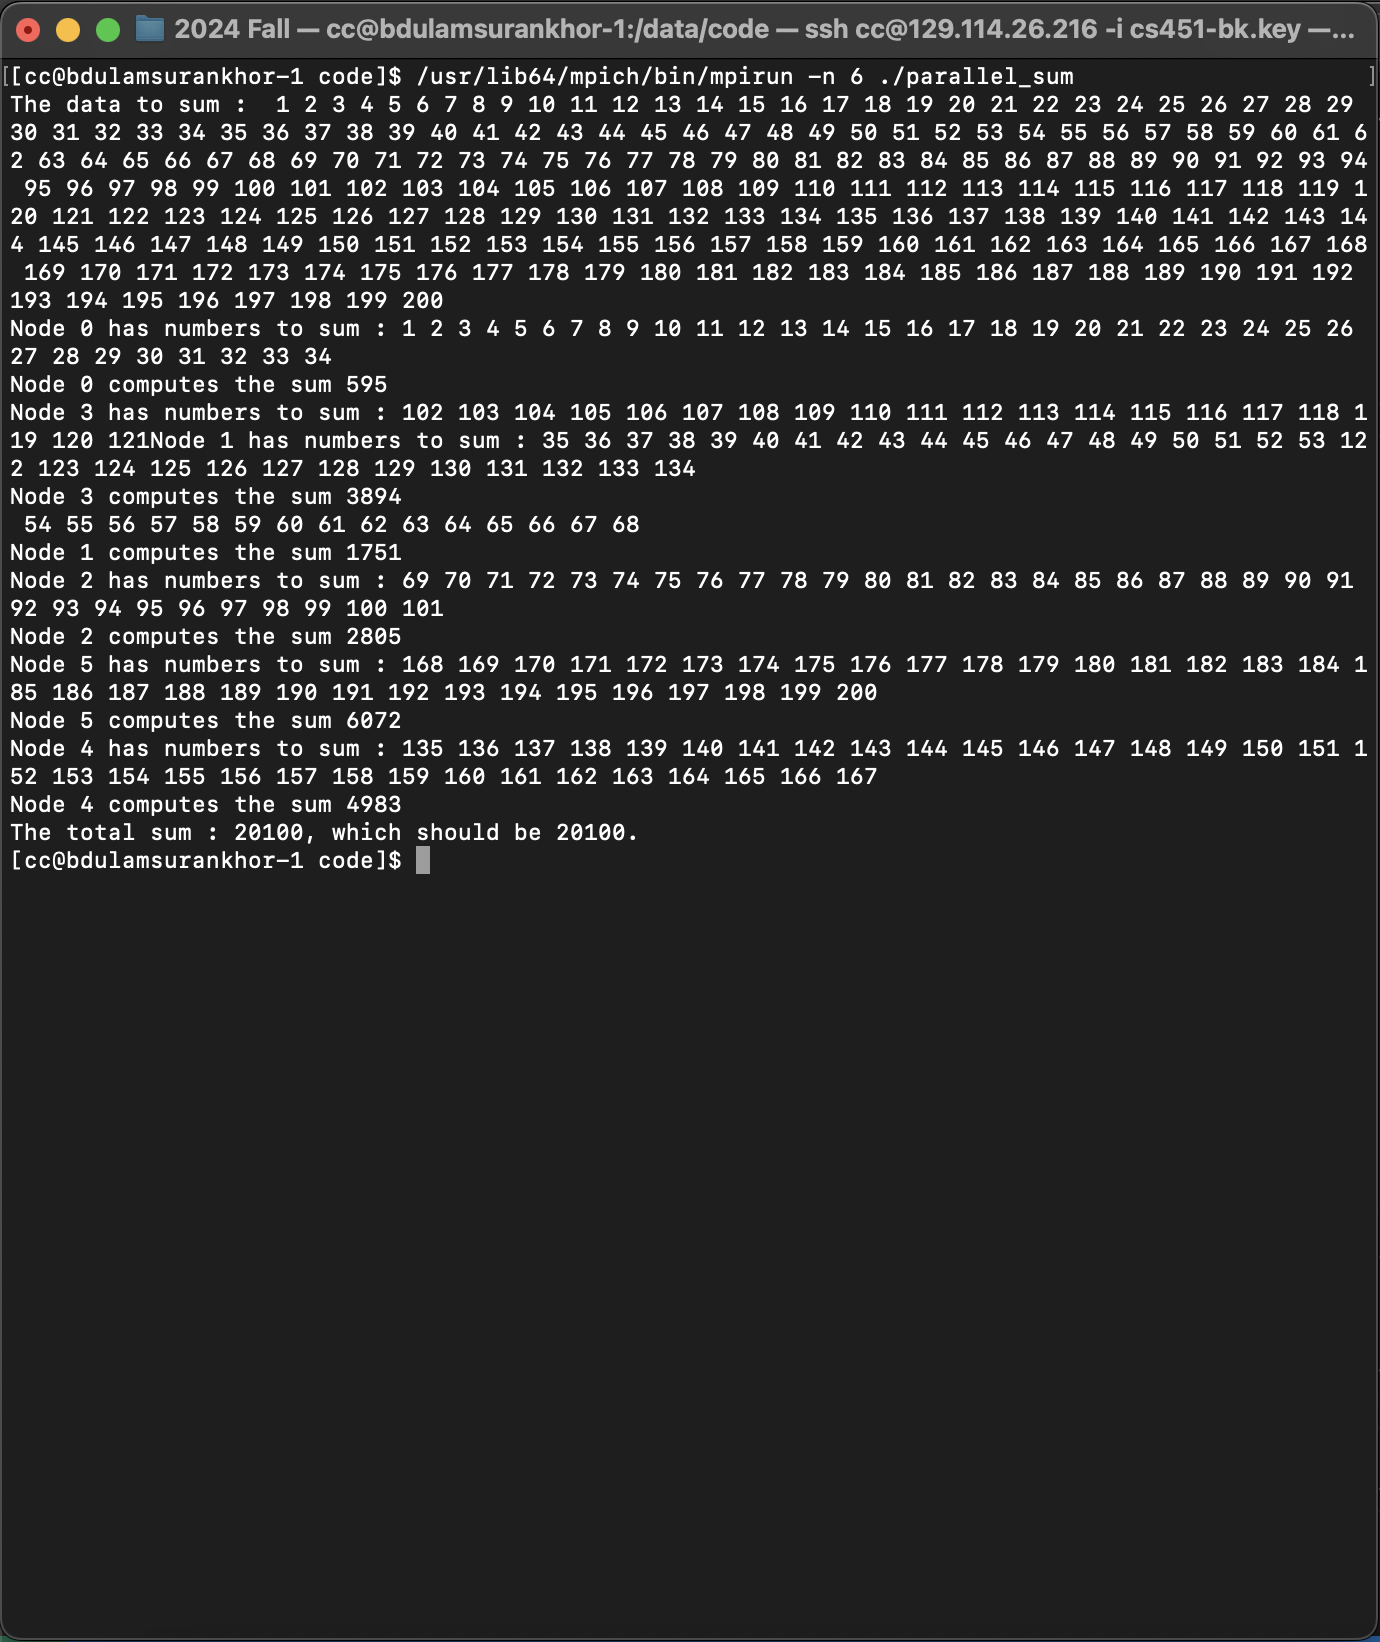
\includegraphics[width=\textwidth]{image14.png}
        \caption{Screenshot of part b, q4. n=6}
      \end{figure}
    \end{enumerate}
  \end{enumerate}
  \item Write up answer the following - a few sentences each:
  \begin{enumerate}
    \item What was the purpose of the NFS server? What happens if you run hello world from a non-shared spot?

    The purpose of the NFS server is to provide a shared file system across the nodes.
    This ensures consistency of data shared between mpi nodes.
    If we run mpi hello world from a non-shared spot, nodes can't access the same file directly, and might attempt to ru an independent instance of the program from their local storage.

    \item How are the different instances of the same program communicating?

    They communicate through message-passing using functions: MPI\_Send, MPI\_Recv and MPI\_Reduce etc.
    MPI\_Send and MPI\_Recv is used for point-to-point communication.
    These functions manage data transfer between nodes and ensure that all processes are synchronized for their tasks.

    \item How might the interconnect effect the speed of a MPI program?

    The network connection between nodes significantly affects the speed of MPI program.
    Because MPI relies on data communication between processes running on different nodes.
    Bandwidth, Latency, Congestion and Overheads have direct impact on the performance of the MPI program.
  \end{enumerate}

\end{enumerate}

\end{document}